\documentclass[12pt,a4paper]{report}
\usepackage{vntex} % Tiếng Việt
\usepackage{graphicx} % Chèn hình ảnh
\usepackage{fancyhdr} % Gói hỗ trợ tạo header và footer fancy
\usepackage{changepage} % Thay đổi lề

% Chèn code
\usepackage{listings} % Thêm gói listings để chèn code
\usepackage{xcolor} % Màu cho code
% Định nghĩa màu sắc
\definecolor{codeblue}{RGB}{0, 0, 255}
\definecolor{codered}{RGB}{255, 0, 0}
\definecolor{codegray}{RGB}{128, 128, 128}
\definecolor{codeblack}{RGB}{0, 0, 0}
\definecolor{lightgray}{RGB}{245, 245, 245}
\definecolor{codecyan}{RGB}{0, 255, 255}

\lstdefinelanguage{javascript}{
    keywords={import, from, const, let, var, function, return, if, else, for, while, do, switch, case, break, continue, new, try, catch, throw, typeof, instanceof, void, with, async, await},
    keywordstyle=\color{codeblue}\bfseries,
    ndkeywords={class, export, default, extends, static, get, set},
    ndkeywordstyle=\color{codeblue}\bfseries,
    identifierstyle=\color{codeblack},
    sensitive=true,
    comment=[l]{//},
    morecomment=[s]{/*}{*/},
    commentstyle=\color{codegray}\itshape,
    stringstyle=\color{codered},
    morestring=[b]",
    morestring=[b]'
}

% Cấu hình listings với màu sắc
\lstset{
    basicstyle=\ttfamily\small,
    keywordstyle=\color{codeblue}\bfseries,
    stringstyle=\color{codered},
    commentstyle=\color{codegray}\itshape,
    numbers=left,
    numberstyle=\tiny\color{codegray},
    stepnumber=1,
    numbersep=5pt,
    showspaces=false,
    showstringspaces=false,
    frame=single,
    framerule=1pt,
    rulecolor=\color{codecyan},
    backgroundcolor=\color{lightgray},
    breaklines=true,
    breakatwhitespace=true,
    tabsize=2,
    captionpos=b,
    language=javascript
}

% Footnote and References
\usepackage[style=numeric,backend=biber]{biblatex} % Sử dụng gói biblatex
\usepackage{capt-of} %  Footnote trong caption
\usepackage[perpage]{footmisc} % Đánh số lại chú thích mỗi trang
\usepackage[toc,page]{appendix}

% Thiết lập bảng
\usepackage{array} % Gói hỗ trợ các bảng phức tạp
\usepackage{tabularx}
\usepackage{longtable} % Tạo bảng qua nhiều trang
\usepackage{cellspace}
\usepackage{diagbox} % Gói hỗ trợ tạo các ô chéo trong bảng
\usepackage{multirow}

% Thiết lập công thức toán học
\usepackage{amsmath} % Gói hỗ trợ các công thức toán học
\usepackage{amsfonts} % Gói hỗ trợ các ký hiệu toán học
\usepackage{amssymb} % Gói hỗ trợ các ký hiệu toán học
\usepackage{graphicx} % Gói hỗ trợ chèn hình ảnh
\usepackage{bm} % Chữ in đậm trong công thức toán 

% Thiết lập khác
\usepackage{tikz}
\usepackage{color}
\usepackage{subcaption}
\usepackage{framed}
\usepackage{float} % Để chèn hình ảnh vào đúng vị trí
\usepackage{fancyvrb} % Đưa dữ liệu dạng nguyên thủy vào


% Thiết lập kích thước
\usepackage{geometry}
\geometry{
    left=3cm,
    right=2cm,
    top=2.5cm,
    bottom=2.5cm,
}
\usepackage{hyperref} %Chèn link
\hypersetup{urlcolor=black,linkcolor=black,citecolor=black,colorlinks=true} % Màu cho các đường nét
\everymath{\color{black}}
\setlength{\headheight}{40pt}
\pagestyle{fancy}


%Header
\fancyhead{} % clear all header fields
\fancyhead[L]{
 \begin{tabular}{rl}
    \begin{picture}(25,15)(0,0)
    \put(0,-8){
\includegraphics[width=12mm, height=12mm]{pictures/IUD_Logo.jpg}}
    %\put(0,-8){\epsfig{width=10mm,figure=hcmut.eps}}
   \end{picture}&
	%\includegraphics[width=8mm, height=8mm]{hcmut.png} & %
	\begin{tabular}{l}
		\textbf{\bf \ttfamily Trường Đại Học Bách Khoa - ĐHQG TP.Hồ Chí Minh}\\
		\textbf{\bf \ttfamily UID LAB}\\
	\end{tabular} 	
 \end{tabular}
}
\fancyhead[R]{
	{\tiny \bf \quad} % Khoảng trắng nhỏ trong header bên phải
}

%Footer
\fancyfoot{} % clear all footer fields
\fancyfoot[L]{\scriptsize \ttfamily IOT WEBSERVER}
\fancyfoot[R]{\scriptsize \ttfamily Trang {\thepage}/86}
\renewcommand{\headrulewidth}{0.3pt}
\renewcommand{\footrulewidth}{0.3pt}

\begin{document}
    \begin{titlepage}   
    \begin{center}
        \vspace*{-2cm} 
        \large
        \textbf{ĐẠI HỌC QUỐC GIA THÀNH PHỐ HỒ CHÍ MINH \\
        TRƯỜNG ĐẠI HỌC BÁCH KHOA\\
        UID LAB\\}
        \vspace{0.5cm}
        
\includegraphics[width=90mm, height=70mm]{pictures/IUD_Logo.jpg} \\
        \rule{\linewidth}{0.5mm}\\
        \vspace{1cm}
        \LARGE
        \textbf{Báo cáo nghiên cứu}\\
        \vspace*{0.5cm}
        \Huge
        \textbf{IOT WEBSERVER}\\
        \vspace{0.5cm}
        \rule{\linewidth}{0.5mm}\\
        \vspace{0.8cm}
        \vspace{1cm}
        \large
        NGƯỜI THỰC HIỆN: VÕ HỮU DƯ\\[0.5cm]
    \end{center}
        
    \vfill
    \large
    \begin{center}
        TP.HCM, \today
    \end{center}
\end{titlepage}
    \tableofcontents  
    \newpage
    \chapter{CẤU TRÚC TỔNG QUAN}
    \section{Chức năng tổng quan}
        \begin{itemize}
            \item Tạo mô hệ thống WebServer giám sát và điều khiển thiết bị IOT từ xa. Cho phép người dùng đăng nhập vào hệ thống và thực hiện các thao tác điều khiển thiết bị IOT.
            \item Lưu trữ dữ liệu từ thiết bị IOT lên WebServer. Tạo giao diện tương tác với người dùng.
            \item Đóng gói WebServer thành một ứng dụng có thể chạy trên nhiều nền tảng khác nhau.
        \end{itemize}
    \section{Sơ đồ khối}
        \begin{figure}[H]
            \centering
            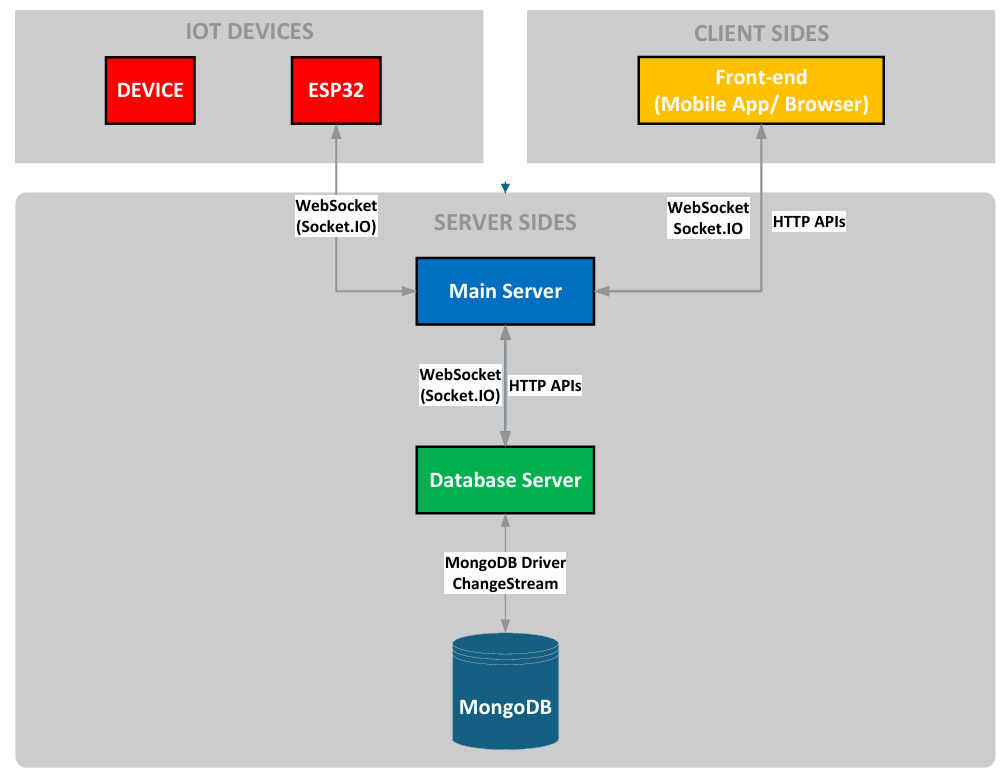
\includegraphics[width=1\textwidth]{pictures/OverviewDiagram.png}
            \caption{Sơ đồ khối WebServer}
            \label{fig:overview_diagram} 
        \end{figure}
        \begin{itemize}
            \item \textbf{ESP32}: thiết bị trung gian, nhận dữ liệu từ thiết bị IOT và gửi dữ liệu lên WebServer.
            \item \textbf{Front-end}: gửi POST/GET request đến WebServer để hiển thị giao diện tương tác với người dùng. 
            \item \textbf{MainServer}: là máy chủ chính của hệ thống, nhận dữ liệu từ ESP32, xác thực dữ liệu và chuyển tiếp dữ liệu đến DatabaServer. Nhận các yêu cầu từ Front-end và trả về dữ liệu cho Front-end.
            \item \textbf{DatabaseServer}: là máy chủ cơ sở dữ liệu, lưu trữ dữ liệu của hệ thống thông qua Database. Nhận yêu cầu từ MainServer và trả về dữ liệu cho MainServer.
            \item \textbf{Database}: là nơi lưu trữ dữ liệu của hệ thống, cho phép truy vấn và lưu dữ liệu từ DatabaseServer.
         \end{itemize}

    \chapter{FRONT END}
    \section{Giới thiệu}
        \begin{itemize}
            \item Front-end là phần giao diện người dùng của hệ thống, cho phép người dùng tương tác với hệ thống thông qua các thao tác trên giao diện.
            \item Front-end được xây dựng bằng Vite, ReactJS, Material UI, Axios và sử dụng WebSocket để nhận dữ liệu từ WebServer. 
            \item Front-end sẽ gửi các yêu cầu đến WebServer để lấy dữ liệu và hiển thị lên giao diện.
        \end{itemize}
    \section{Cài đặt}
        \begin{itemize}
            \item Cài đặt NodeJS và NPM trên máy tính của bạn. Bạn có thể tải NodeJS tại địa chỉ: \url{https://nodejs.org/en/download/}
            \item Cài đặt Vite bằng lệnh sau:
                \begin{lstlisting}
    npm create vite@latest
                \end{lstlisting}
                Chọn Framework là React và variant là Javascript.
            \item Chạy ứng dụng bằng lệnh sau:
                \begin{lstlisting}
    npm run dev
                \end{lstlisting}
            \item Mở trình duyệt và truy cập vào địa chỉ: \url{http://localhost:5173/}
        \end{itemize}
    \section{Bố cục giao diện}
        Giao diện có dạng dashboard được phân bố như hình:
        \begin{figure}[H]
            \centering
            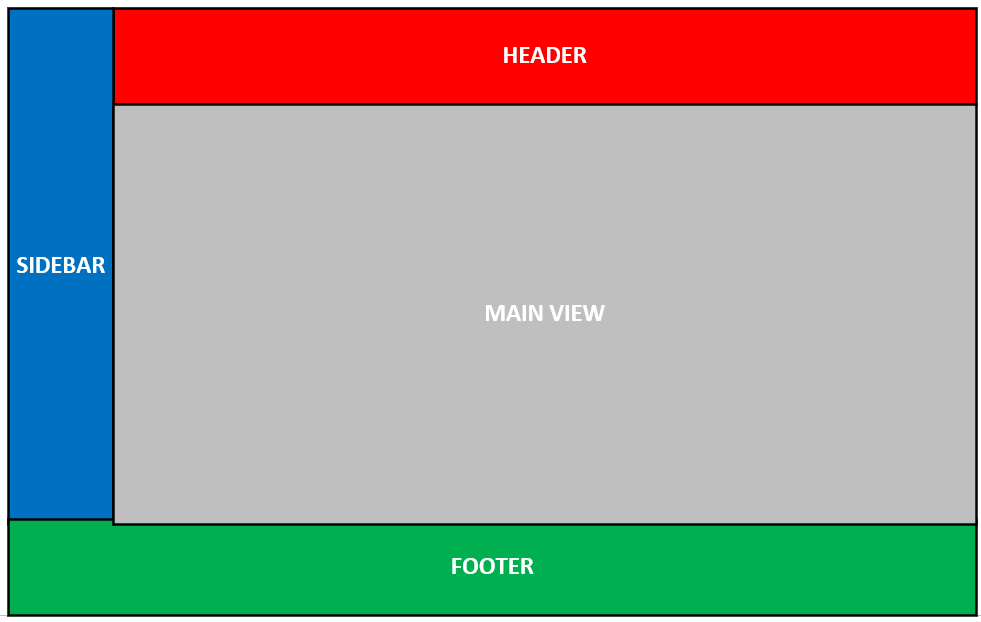
\includegraphics[width=0.8\textwidth]{pictures/dashboard.png}
            \caption{Giao diện dashboard}
            \label{fig:dashboard}
        \end{figure}
    \section{Cấu trúc thư mục}
        \begin{itemize}
            \item \textbf{node\_modules}: Thư mục chứa các thư viện được cài đặt bằng NPM.
            \item \textbf{public}: Thư mục chứa các tệp tĩnh như hình ảnh, biểu tượng, v.v.
            \item \textbf{src}: Thư mục chứa mã nguồn của ứng dụng.
                \begin{itemize}
                    \item \textbf{api}: Thư mục chứa các tệp API của ứng dụng.
                    \item \textbf{assets}: Thư mục chứa các tệp tài nguyên như hình ảnh, biểu tượng, v.v.
                    \item \textbf{components}: Thư mục chứa các thành phần giao diện của ứng dụng: Header.jsx, Footer.jsx, Sidebar.jsx.
                    \item \textbf{hooks}: Thư mục chứa các hook tùy chỉnh của ứng dụng, hiển thị ở phần Main view.
                    \item \textbf{pages}: Thư mục chứa các trang của ứng dụng.
                    \item \textbf{router}: Thư mục chứa các tệp định tuyến của ứng dụng.
                    \item \textbf{services}: Thư mục chứa các tệp dịch vụ của ứng dụng.
                    \item \textbf{styles}: Thư mục chứa các tệp CSS của ứng dụng.
                    \item \textbf{App.jsx}: Tệp chính của ứng dụng.
                    \item \textbf{main.jsx}: Tệp khởi động ứng dụng.
                    \item \textbf{theme.js}: Tệp chứa định dạng nền cho ứng dụng.
                \end{itemize}
        \end{itemize}
    \section{Cài đặt thư viện}
        \begin{itemize}
            \item Thư viện Material UI: Thư viện giao diện người dùng cho React.
            \begin{lstlisting}
    npm install @mui/material
            \end{lstlisting} 
            \item Thư viện Axios: Thư viện gửi yêu cầu HTTP.
            \begin{lstlisting}
    npm install axios
            \end{lstlisting} 
            \item Thư viện React Router: Thư viện định tuyến cho React.
            \begin{lstlisting}
    npm install react-router-dom
            \end{lstlisting}
            \item Thư viện Socket Clint: Thư viện WebSocket cho Front
            \begin{lstlisting}
    npm install socket.io-client
            \end{lstlisting}
            \item Các thư viện khác cài đặt trong quá trình phát triển.
        \end{itemize}
    \section{COMPONENTS}
        \subsection{Header}
            \hspace*{0.6cm}Header là thành phần hiển thị tiêu đề của ứng dụng, thanh tìm kiếm, thông tin người dùng.
            \begin{figure}[H]
                \centering
                
\includegraphics[width=1\textwidth]{pictures/Header_1.png}
                \caption{Giao diện Header trước khi Login}
                \label{fig:header}
            \end{figure}
            \begin{figure}[H]
                \centering
                
\includegraphics[width=1\textwidth]{pictures/Header_2.png}
                \caption{Giao diện Header sau khi Login}
                \label{fig:header}
            \end{figure}
            \subsubsection{Kết nối Socket}
                \hspace*{0.6cm}Socket.IO được sử dụng để giao tiếp thời gian thực với server:
                \begin{lstlisting}
    const API_URL = import.meta.env.VITE_API_URL || "http://localhost:5000";
    const socket = io(API_URL, {
        reconnection: true,
        reconnectionAttempts: 5,
        reconnectionDelay: 1000,
        transports: ["websocket", "polling"],
        auth: { token: document.cookie.split("; ").find(row => row.startsWith("authToken="))?.split("=")[1] || null }
    });
                \end{lstlisting}
                \begin{itemize}
                    \item \texttt{API\_URL}: Lấy từ biến môi trường hoặc mặc định là \texttt{http://localhost:5000}.
                    \item \texttt{socket}: Kết nối với server, ưu tiên WebSocket, dùng polling nếu thất bại. Có cơ chế tự động thử lại 5 lần, cách nhau 1 giây. Token xác thực được lấy từ cookie.
                \end{itemize}

            \subsubsection{Thành Phần Giao Diện Tùy Chỉnh}
                \hspace*{0.6cm}Thanh tìm kiếm được định kiểu bằng \texttt{styled}:
                \begin{lstlisting}
    const Search = styled("div")(({ theme }) => ({
        position: "relative",
        borderRadius: theme.shape.borderRadius,
        backgroundColor: alpha(theme.palette.text.primary, 0.05),
        "&:hover": {
        backgroundColor: alpha(theme.palette.text.primary, 0.1),
        },
        marginLeft: theme.spacing(2),
        width: "100%",
        maxWidth: 300,
    }));
    const SearchIconWrapper = styled("div")(({ theme }) => ({
        padding: theme.spacing(0, 2),
        height: "100%",
        position: "absolute",
        display: "flex",
        alignItems: "center",
        justifyContent: "center",
        color: theme.palette.text.secondary,
    }));
    const StyledInputBase = styled(InputBase)(({ theme }) => ({
        color: theme.palette.text.primary,
        paddingLeft: `calc(1em + ${theme.spacing(4)})`,
        width: "100%",
    }));
                \end{lstlisting}
                \begin{itemize}
                    \item \texttt{Search}: Container thanh tìm kiếm, nền mờ (5\% độ mờ), hover đổi thành 10\%, rộng tối đa 300px.
                    \item \texttt{SearchIconWrapper}: Định vị icon tìm kiếm bên trái, căn giữa.
                    \item \texttt{StyledInputBase}: Ô nhập liệu có màu chữ theo theme, thêm padding để tránh che icon.
                \end{itemize}

            \subsubsection{Component Header}
                \hspace*{0.6cm}Component nhận các props:
                \begin{lstlisting}
    const Header = ({ onToggleSidebar, user, setUser }) => {}
                \end{lstlisting}
                \begin{itemize}
                    \item \texttt{onToggleSidebar}: Hàm mở/đóng sidebar.
                    \item \texttt{user}: Thông tin người dùng (null nếu chưa đăng nhập).
                    \item \texttt{setUser}: Cập nhật trạng thái người dùng.
                \end{itemize}

            \subsubsection{Trạng Thái và Hook}
                \begin{lstlisting}
    const theme = useTheme();
    const [anchorEl, setAnchorEl] = useState(null);
    const { email, setEmail, password, setPassword, openLogin, setOpenLogin, handleLogin, handleLogout } = useAuth(setUser, socket);
                \end{lstlisting}
                \begin{itemize}
                    \item \texttt{theme}: Lấy theme để tạo kiểu.
                    \item \texttt{anchorEl}: Lưu vị trí mở \texttt{AvatarMenu}.
                    \item \texttt{useAuth}: Cung cấp trạng thái (email, password, openLogin) và hàm xử lý đăng nhập/đăng xuất.
                \end{itemize}

            \subsubsection{Xử Lý Sự Kiện}
                \begin{lstlisting}
    const handleAvatarClick = (event) => {
        setAnchorEl(event.currentTarget);
    };
    const handleMenuClose = () => {
        setAnchorEl(null);
    };
                \end{lstlisting}
                \begin{itemize}
                    \item \texttt{handleAvatarClick}: Mở \texttt{AvatarMenu} khi click avatar.
                    \item \texttt{handleMenuClose}: Đóng menu.
                \end{itemize}

            \subsubsection{URL Ảnh Đại Diện}
                \begin{lstlisting}
    const avatarSrc = user?.avatar ? `${API_URL}${user.avatar}` : undefined;
    console.log("Avatar URL in Header:", avatarSrc);
                \end{lstlisting}
                Tạo URL ảnh đại diện bằng cách nối \texttt{API\_URL} với đường dẫn avatar, in ra để debug.

            \subsubsection{Cấu Trúc JSX}
                \hspace*{0.6cm}Thanh điều hướng chính:
                \begin{lstlisting}
    <AppBar
        position="fixed"
        sx={{
            backgroundColor: theme.palette.background.header,
            color: theme.palette.text.primary,
            zIndex: theme.zIndex.drawer + 1,
            boxShadow: "none",
        }}
    >
                \end{lstlisting}
                \begin{itemize}
                    \item \texttt{AppBar}: Thanh cố định, màu nền và chữ theo theme, z-index cao, không có bóng.
                \end{itemize}

                Phần trái của \texttt{Toolbar}:
                \begin{lstlisting}
        <Toolbar sx={{ display: "flex", justifyContent: "space-between", pl: "0px" }}>
            <Box sx={{ display: "flex", alignItems: "center" }}>
                <IconButton color="inherit" onClick={onToggleSidebar} sx={{ mr: 2, p: 0 }}>
                    <MenuIcon />
                </button>
                <img src="/logo.png" alt="logo" style={{ width: 60, height: 60, marginRight: 10 }} />
                <Typography variant="h6" fontWeight="bold">
                    UID LAB
                </Typography>
            </Box>
                \end{lstlisting}
                \begin{itemize}
                    \item Nút \texttt{MenuIcon} mở/đóng sidebar.
                    \item Logo (60x60px) và tiêu đề "UID LAB" kiểu h6, in đậm.
                \end{itemize}

                Phần phải (thanh tìm kiếm và xác thực):
                \begin{lstlisting}
            <Box sx={{ display: "flex", alignItems: "center", gap: 2 }}>
                <Search>
                    <SearchIconWrapper>
                        <SearchIcon />
                    </SearchIconWrapper>
                    <StyledInputBase
                        placeholder="Search..."
                        inputProps={{ "aria-label": "search" }}
                    />
                </Search>
                {!user ? (
                    <Typography
                        color="inherit"
                        onClick={() => setOpenLogin(true)}
                        sx={{ cursor: "pointer" }}
                    >
                        Dang Nhap
                    </Typography>
                ) : (
                    <Box sx={{ display: "flex", alignItems: "center", gap: 1 }}>
                        <Avatar
                            src={avatarSrc}
                            alt={user.username}
                            onClick={handleAvatarClick}
                            sx={{ cursor: "pointer", width: 40, height: 40 }}
                        />
                        <AvatarMenu
                            anchorEl={anchorEl}
                            onClose={handleMenuClose}
                            user={user}
                            setUser={setUser}
                            onLogout={handleLogout}
                        />
                    </Box>
                )}
            </Box>
                \end{lstlisting}
                \begin{itemize}
                    \item Thanh tìm kiếm: Ô nhập liệu với icon và placeholder.
                    \item Xác thực: Hiển thị link "Đăng nhập" nếu chưa đăng nhập, hoặc avatar và \texttt{AvatarMenu} nếu đã đăng nhập.
                \end{itemize}

                Modal đăng nhập:
                \begin{lstlisting}
            <LoginDialog
                open={openLogin}
                onClose={() => setOpenLogin(false)}
                email={email}
                setEmail={setEmail}
                password={password}
                setPassword={setPassword}
                handleLogin={handleLogin}
            />
                \end{lstlisting}
                \begin{itemize}
                    \item \texttt{LoginDialog}: Modal đăng nhập, hiển thị khi \texttt{openLogin} là true.
                \end{itemize}
            \subsubsection{Chức năng chính}
                \begin{itemize}
                    \item \textbf{Mở/đóng Sidebar}: Click \texttt{MenuIcon} gọi \texttt{onToggleSidebar}.
                    \item \textbf{Thanh Tìm Kiếm}: Ô nhập liệu với icon và kiểu dáng tùy chỉnh.
                    \item \textbf{Xác Thực Người Dùng}:
                    \begin{itemize}
                        \item Chưa đăng nhập: Link "Đăng nhập" mở \texttt{LoginDialog}.
                        \item Đã đăng nhập: Avatar mở \texttt{AvatarMenu} với tùy chọn hồ sơ/đăng xuất.
                    \end{itemize}
                    \item \textbf{Giao Tiếp Thời Gian Thực}: Socket.IO duy trì kết nối với server, hỗ trợ xác thực qua token.
                \end{itemize}
        \subsection{LoginDialog}
            \hspace*{0.6cm}Là một hộp thoại (modal), sử dụng Material-UI để tạo giao diện đăng nhập người dùng. Nó hiển thị một biểu mẫu với các trường nhập email, mật khẩu và nút đăng nhập.
            \begin{figure}[H]
                \centering
                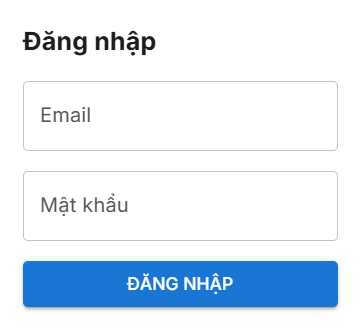
\includegraphics[width=0.5\textwidth]{pictures/LoginDialog.png}
                \caption{Giao diện LoginDialog}
                \label{fig:login}
            \end{figure}
            \subsubsection{Import}
                \hspace*{0.6cm}Các thư viện và thành phần Material-UI được nhập để xây dựng giao diện:
                \begin{lstlisting}
    import React from 'react';
    import { Dialog, Box, Typography, TextField, Button } from '@mui/material';
                \end{lstlisting}
                \begin{itemize}
                    \item \texttt{React}: Thư viện chính để xây dựng component.
                    \item \texttt{Material-UI}: Cung cấp các thành phần:
                    \begin{itemize}
                        \item \texttt{Dialog}: Hộp thoại hiển thị biểu mẫu đăng nhập.
                        \item \texttt{Box}: Container để sắp xếp bố cục.
                        \item \texttt{Typography}: Hiển thị tiêu đề.
                        \item \texttt{TextField}: Trường nhập liệu cho email và mật khẩu.
                        \item \texttt{Button}: Nút thực hiện hành động đăng nhập.
                    \end{itemize}
                \end{itemize}

            \subsubsection{Component LoginDialog}
                \hspace*{0.6cm}Component nhận các props để quản lý trạng thái và xử lý đăng nhập:
                \begin{lstlisting}
    const LoginDialog = ({ open, onClose, email, setEmail, password, setPassword, handleLogin }) => {
                \end{lstlisting}
                \begin{itemize}
                    \item \texttt{open}: Trạng thái hiển thị của hộp thoại (true/false).
                    \item \texttt{onClose}: Hàm đóng hộp thoại.
                    \item \texttt{email}, \texttt{setEmail}: Giá trị và hàm cập nhật email.
                    \item \texttt{password}, \texttt{setPassword}: Giá trị và hàm cập nhật mật khẩu.
                    \item \texttt{handleLogin}: Hàm xử lý logic đăng nhập.
                \end{itemize}

            \subsubsection{Cấu Trúc JSX}
                \hspace*{0.6cm}Giao diện của \texttt{LoginDialog} được định nghĩa trong JSX:
                \begin{lstlisting}
    return (
        <Dialog open={open} onClose={onClose}>
            <Box sx={{ p: 3, display: 'flex', flexDirection: 'column', gap: 2, width: 300 }}>
                <Typography variant="h6" fontWeight="bold">Dang nhap</Typography>
                <TextField
                    label="Email"
                    value={email}
                    onChange={(e) => setEmail(e.target.value)}
                    fullWidth
                />
                <TextField
                    label="Mat khau"
                    type="password"
                    value={password}
                    onChange={(e) => setPassword(e.target.value)}
                    fullWidth
                />
                <Button variant="contained" onClick={handleLogin}>
                    Dang nhap
                </Button>
            </Box>
        </Dialog>
    );
                \end{lstlisting}
                \begin{itemize}
                    \item \texttt{Dialog}: Hộp thoại được điều khiển bởi \texttt{open} và \texttt{onClose}.
                    \item \texttt{Box}: Container với:
                    \begin{itemize}
                        \item Padding 3 đơn vị (\texttt{p: 3}).
                        \item Bố cục cột dọc (\texttt{flexDirection: 'column'}).
                        \item Khoảng cách giữa các phần tử (\texttt{gap: 2}).
                        \item Chiều rộng cố định 300px (\texttt{width: 300}).
                    \end{itemize}
                    \item \texttt{Typography}: Tiêu đề "Đăng nhập" với kiểu \texttt{h6}, in đậm.
                    \item \texttt{TextField} (Email): Trường nhập liệu email, liên kết với \texttt{email} và \texttt{setEmail}, chiếm toàn bộ chiều rộng (\texttt{fullWidth}).
                    \item \texttt{TextField} (Mật khẩu): Trường nhập liệu mật khẩu, loại \texttt{password} để ẩn ký tự, liên kết với \texttt{password} và \texttt{setPassword}.
                    \item \texttt{Button}: Nút "Đăng nhập" với kiểu \texttt{contained} (nút nổi), gọi \texttt{handleLogin} khi click.
                \end{itemize}

            \subsubsection{Export}
                \hspace*{0.6cm}Component được xuất để sử dụng trong các phần khác của ứng dụng:
                \begin{lstlisting}
    export default LoginDialog;
                \end{lstlisting}
            \subsubsection{Chức Năng Chính}
                \begin{itemize}
                    \item \textbf{Hiển thị Hộp Thoại Đăng Nhập}: Hộp thoại xuất hiện khi \texttt{open} là \texttt{true}, đóng khi gọi \texttt{onClose}.
                    \item \textbf{Nhập Thông Tin Đăng Nhập}: Người dùng nhập email và mật khẩu vào các trường \texttt{TextField}, dữ liệu được cập nhật qua \texttt{setEmail} và \texttt{setPassword}.
                    \item \textbf{Xử Lý Đăng Nhập}: Nút "Đăng nhập" gọi \texttt{handleLogin} để thực hiện xác thực (logic cụ thể phụ thuộc vào hàm này).
                    \item \textbf{Giao Diện}: Sử dụng Material-UI để tạo bố cục rõ ràng, trực quan, với các trường nhập liệu và nút được sắp xếp gọn gàng.
                \end{itemize}
        \subsection{AvatarMenu}
            \hspace*{0.6cm}Là một menu sử dụng Material-UI để hiển thị các tùy chọn cho người dùng đã đăng nhập, bao gồm cập nhật avatar, đổi mật khẩu và đăng xuất. Nó tích hợp với API thông qua \texttt{axios} và sử dụng \texttt{SnackbarContext} để hiển thị thông báo.
            \begin{figure}[H]
                \centering
                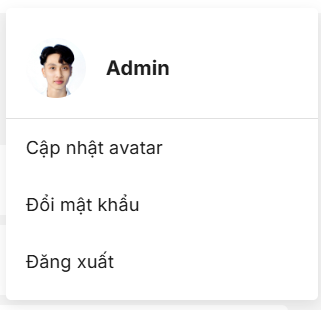
\includegraphics[width=0.5\textwidth]{pictures/AvatarMenu.png}
                \caption{Giao diện AvatarMenu}
                \label{fig:avatar}
            \end{figure}
            \subsubsection{Import}
                \hspace*{0.6cm}Các thư viện và thành phần được nhập để xây dựng \texttt{AvatarMenu}:
                \begin{lstlisting}
    import React, { useState } from "react";
    import {
        Avatar, Menu, MenuItem, Divider, Box, Typography, useTheme,
    } from "@mui/material";
    import axios from "axios";
    import ChangePasswordDialog from "./ChangePasswordDialog";
    import { useSnackbar } from '../context/SnackbarContext';
                \end{lstlisting}
                \begin{itemize}
                    \item \texttt{React}, \texttt{useState}: Quản lý trạng thái cục bộ.
                    \item \texttt{Material-UI}: Cung cấp các thành phần:
                    \begin{itemize}
                        \item \texttt{Avatar}: Hiển thị ảnh đại diện.
                        \item \texttt{Menu}, \texttt{MenuItem}: Tạo menu ngữ cảnh.
                        \item \texttt{Divider}: Đường phân cách.
                        \item \texttt{Box}, \texttt{Typography}: Sắp xếp bố cục và hiển thị văn bản.
                        \item \texttt{useTheme}: Lấy theme ứng dụng.
                    \end{itemize}
                    \item \texttt{axios}: Gửi yêu cầu HTTP tới API.
                    \item \texttt{ChangePasswordDialog}: Component để đổi mật khẩu.
                    \item \texttt{useSnackbar}: Hook từ \texttt{SnackbarContext} để hiển thị thông báo.
                \end{itemize}

            \subsubsection{API URL}
                \hspace*{0.6cm}Định nghĩa URL API:
                \begin{lstlisting}
    const API_URL = import.meta.env.VITE_API_URL || "http://localhost:5000";
                \end{lstlisting}
                \begin{itemize}
                    \item \texttt{API\_URL}: Lấy từ biến môi trường hoặc mặc định là \texttt{http://localhost:5000}.
                \end{itemize}

            \subsubsection{Component AvatarMenu}
                \hspace*{0.6cm}Component nhận các props:
                \begin{lstlisting}
    const AvatarMenu = ({ anchorEl, onClose, user, setUser, onLogout }) => {
                \end{lstlisting}
                \begin{itemize}
                    \item \texttt{anchorEl}: Vị trí neo menu.
                    \item \texttt{onClose}: Hàm đóng menu.
                    \item \texttt{user}: Thông tin người dùng (username, avatar).
                    \item \texttt{setUser}: Cập nhật trạng thái người dùng.
                    \item \texttt{onLogout}: Hàm xử lý đăng xuất.
                \end{itemize}

            \subsubsection{Trạng Thái}
                \hspace*{0.6cm}Quản lý trạng thái cục bộ:
                \begin{lstlisting}
    const theme = useTheme();
    const [openChangePassword, setOpenChangePassword] = useState(false);
    const [oldPassword, setOldPassword] = useState("");
    const [newPassword, setNewPassword] = useState("");
    const { showSnackbar } = useSnackbar();
                \end{lstlisting}
                \begin{itemize}
                    \item \texttt{theme}: Lấy theme để tạo kiểu.
                    \item \texttt{openChangePassword}: Điều khiển hiển thị \texttt{ChangePasswordDialog}.
                    \item \texttt{oldPassword}, \texttt{newPassword}: Lưu mật khẩu cũ và mới.
                    \item \texttt{showSnackbar}: Hàm hiển thị thông báo từ \texttt{SnackbarContext}.
                \end{itemize}

            \subsubsection{Xử Lý Cập Nhật Avatar}
                \hspace*{0.6cm}Hàm xử lý tải lên avatar:
                \begin{lstlisting}
    const handleAvatarChange = async (event) => {
        const file = event.target.files[0];
        if (file) {
            const formData = new FormData();
            formData.append("avatar", file);
            try {
                const res = await axios.post(
                    `${import.meta.env.VITE_API_URL}/api/users
                    /update-avatar`,
                    formData,
                    { withCredentials: true }
                );
                const updatedAvatar = res.data.avatar;
                setUser((prev) => ({ ...prev, avatar: updatedAvatar }));
                localStorage.setItem("user", JSON.stringify({ username: user.username, avatar: updatedAvatar }));
                showSnackbar("Update avatar successful", "success");
                onClose();
            } catch (error) {
                console.error("Error when updating avatar:", error);
                showSnackbar("Error when updating avatar", "error");
            }
        }
    };
                \end{lstlisting}
                \begin{itemize}
                    \item Lấy tệp ảnh từ \texttt{event.target.files}.
                    \item Tạo \texttt{FormData} để gửi tệp lên API \texttt{/api/users/update-avatar}.
                    \item Cập nhật trạng thái \texttt{user} và \texttt{localStorage} nếu thành công.
                    \item Hiển thị thông báo bằng \texttt{showSnackbar}.
                    \item Xử lý lỗi với thông báo lỗi.
                \end{itemize}

            \subsubsection{Xử Lý Đổi Mật Khẩu}
                \hspace*{0.6cm}Hàm xử lý đổi mật khẩu:
                \begin{lstlisting}
    const handleChangePassword = async () => {
        try {
            const res = await axios.post(
                `${import.meta.env.VITE_API_URL}/api/users
                /change-password`,
                { oldPassword, newPassword },
                { withCredentials: true }
            );
            showSnackbar(res.data.message, "success");
            setOpenChangePassword(false);
            setOldPassword("");
            setNewPassword("");
        } catch (error) {
            console.error("Error when changing password:", error);
            showSnackbar(error.response?.data?.message || "Error when changing password", "error");
        }
    };
                \end{lstlisting}
                \begin{itemize}
                    \item Gửi yêu cầu POST tới \texttt{/api/users/change-password} với \texttt{oldPassword} và \texttt{newPassword}.
                    \item Hiển thị thông báo thành công và reset trạng thái nếu thành công.
                    \item Hiển thị thông báo lỗi nếu thất bại.
                \end{itemize}

            \subsubsection{Xử Lý Đăng Xuất}
                \hspace*{0.6cm}Hàm xử lý đăng xuất:
                \begin{lstlisting}
    const handleLogoutClick = () => {
        onLogout();
        onClose();
    };
                \end{lstlisting}
                \begin{itemize}
                    \item Gọi \texttt{onLogout} và đóng menu.
                \end{itemize}

            \subsubsection{URL Ảnh Đại Diện}
                \hspace*{0.6cm}Tạo URL cho avatar:
                \begin{lstlisting}
    const avatarSrc = user.avatar ? `${API_URL}${user.avatar}` : undefined;
    console.log("Avatar URL in AvatarMenu:", avatarSrc);
                \end{lstlisting}
                \begin{itemize}
                    \item Nối \texttt{API\_URL} với đường dẫn avatar, in ra để debug.
                \end{itemize}

            \subsubsection{Cấu Trúc JSX}
                \hspace*{0.6cm}Giao diện menu:
                \begin{lstlisting}
    <Menu
        anchorEl={anchorEl}
        open={Boolean(anchorEl)}
        onClose={onClose}
        anchorOrigin={{ vertical: "bottom", horizontal: "right" }}
        transformOrigin={{ vertical: "top", horizontal: "right" }}
        PaperProps={{
            sx: {
                mt: 1,
                width: 250,
                bgcolor: theme.palette.background.paper,
                color: theme.palette.text.primary,
                boxShadow: "0px 4px 12px rgba(0, 0, 0, 0.1)",
            },
        }}
    >
        <Box sx={{ display: "flex", alignItems: "center", p: 2 }}>
            <Avatar
                src={avatarSrc}
                alt={user.username}
                sx={{ mr: 2, width: 48, height: 48 }}
            />
            <Typography variant="subtitle1" fontWeight="bold">
                {user.username}
            </Typography>
        </Box>
        <Divider />
        <MenuItem
            component="label"
            sx={{ py: 1.5, fontSize: "0.9rem" }}
        >
            Update avatar
            <input
                type="file"
                accept="image/*"
                hidden
                onChange={handleAvatarChange}
            />
        </MenuItem>
        <MenuItem
            onClick={() => setOpenChangePassword(true)}
            sx={{ py: 1.5, fontSize: "0.9rem" }}
        >
            Changing Password
        </MenuItem>
        <MenuItem
            onClick={handleLogoutClick}
            sx={{ py: 1.5, fontSize: "0.9rem" }}
        >
            Logout
        </MenuItem>
    </Menu>
                \end{lstlisting}
                \begin{itemize}
                    \item \texttt{Menu}: Menu ngữ cảnh, neo tại \texttt{anchorEl}, hiển thị khi \texttt{anchorEl} tồn tại.
                    \item \texttt{Box}: Hiển thị avatar và tên người dùng, căn chỉnh ngang.
                    \item \texttt{Divider}: Đường phân cách.
                    \item \texttt{MenuItem}:
                    \begin{itemize}
                        \item "Cập nhật avatar": Chứa input file ẩn để tải ảnh.
                        \item "Đổi mật khẩu": Mở \texttt{ChangePasswordDialog}.
                        \item "Đăng xuất": Gọi \texttt{handleLogoutClick}.
                    \end{itemize}
                \end{itemize}

                Hộp thoại đổi mật khẩu:
                \begin{lstlisting}
    <ChangePasswordDialog
        open={openChangePassword}
        onClose={() => {
            setOpenChangePassword(false);
            setOldPassword("");
            setNewPassword("");
        }}
        oldPassword={oldPassword}
        setOldPassword={setOldPassword}
        newPassword={newPassword}
        setNewPassword={setNewPassword}
        handleChangePassword={handleChangePassword}
    />
                \end{lstlisting}
                \begin{itemize}
                    \item \texttt{ChangePasswordDialog}: Hộp thoại hiển thị khi \texttt{openChangePassword} là \texttt{true}.
                \end{itemize}

            \subsubsection{Export}
                \begin{lstlisting}
    export default AvatarMenu;
                \end{lstlisting}
            \subsubsection{Chức Năng Chính}
                \begin{itemize}
                    \item \textbf{Hiển Thị Menu Ngữ Cảnh}: Menu xuất hiện khi click avatar, hiển thị tên người dùng và các tùy chọn.
                    \item \textbf{Cập Nhật Avatar}: Cho phép tải lên ảnh mới, gửi tới API và cập nhật trạng thái người dùng.
                    \item \textbf{Đổi Mật Khẩu}: Mở hộp thoại để nhập mật khẩu cũ/mới, gửi yêu cầu đổi mật khẩu tới API.
                    \item \textbf{Đăng Xuất}: Xử lý đăng xuất và đóng menu.
                    \item \textbf Thông Báo**: Sử dụng \texttt{showSnackbar} để hiển thị thông báo thành công/lỗi.
                \end{itemize}

        \subsection{ChangePasswordDialog}
            \hspace*{0.6cm}Là một hộp thoại (modal) sử dụng Material-UI để hiển thị biểu mẫu đổi mật khẩu cho người dùng. Nó cho phép người dùng nhập mật khẩu cũ và mật khẩu mới, và thực hiện xác thực khi nhấn nút "Đổi mật khẩu".
            \begin{figure}[H]
                \centering
                
\includegraphics[width=0.5\textwidth]{pictures/ChangePasswordDialog.png}
                \caption{Giao diện ChangePasswordDialog}
                \label{fig:change}
            \end{figure}
            \subsubsection{Import}
                \hspace*{0.6cm}Các thư viện và thành phần Material-UI được nhập để xây dựng giao diện:
                \begin{lstlisting}
    import React from "react";
    import { Dialog, Box, Typography, TextField, Button } from "@mui/material";
                \end{lstlisting}
                \begin{itemize}
                    \item \texttt{React}: Thư viện chính để xây dựng component.
                    \item \texttt{Material-UI}: Cung cấp các thành phần:
                    \begin{itemize}
                        \item \texttt{Dialog}: Hộp thoại hiển thị biểu mẫu đổi mật khẩu.
                        \item \texttt{Box}: Container để sắp xếp bố cục.
                        \item \texttt{Typography}: Hiển thị tiêu đề.
                        \item \texttt{TextField}: Trường nhập liệu cho mật khẩu cũ và mới.
                        \item \texttt{Button}: Nút xác nhận hành động đổi mật khẩu.
                    \end{itemize}
                \end{itemize}

            \subsubsection{Component ChangePasswordDialog}
                \hspace*{0.6cm}Component nhận các props để quản lý trạng thái và xử lý đổi mật khẩu:
                \begin{lstlisting}
    const ChangePasswordDialog = ({
        open,
        onClose,
        oldPassword,
        setOldPassword,
        newPassword,
        setNewPassword,
        handleChangePassword,
    }) => {}
                \end{lstlisting}
                \begin{itemize}
                    \item \texttt{open}: Trạng thái hiển thị của hộp thoại (true/false).
                    \item \texttt{onClose}: Hàm đóng hộp thoại.
                    \item \texttt{oldPassword}, \texttt{setOldPassword}: Giá trị và hàm cập nhật mật khẩu cũ.
                    \item \texttt{newPassword}, \texttt{setNewPassword}: Giá trị và hàm cập nhật mật khẩu mới.
                    \item \texttt{handleChangePassword}: Hàm xử lý logic đổi mật khẩu.
                \end{itemize}

            \subsubsection{Cấu Trúc JSX}
                \hspace*{0.6cm}Giao diện của \texttt{ChangePasswordDialog} được định nghĩa trong JSX:
                \begin{lstlisting}
    return (
        <Dialog open={open} onClose={onClose}>
            <Box sx={{ p: 3, display: "flex", flexDirection: "column", gap: 2, width: 300 }}>
                <Typography variant="h6" fontWeight="bold">Change Password</Typography>
                <TextField
                    label="Old Password"
                    type="password"
                    value={oldPassword}
                    onChange={(e) => setOldPassword(e.target.value)}
                    fullWidth
                />
                <TextField
                    label="New Password"
                    type="password"
                    value={newPassword}
                    onChange={(e) => setNewPassword(e.target.value)}
                    fullWidth
                />
                <Button variant="contained" onClick={handleChangePassword}>
                    Validate
                </Button>
            </Box>
        </Dialog>
    );
                \end{lstlisting}
                \begin{itemize}
                    \item \texttt{Dialog}: Hộp thoại được điều khiển bởi \texttt{open} và \texttt{onClose}.
                    \item \texttt{Box}: Container với:
                    \begin{itemize}
                        \item Padding 3 đơn vị (\texttt{p: 3}).
                        \item Bố cục cột dọc (\texttt{flexDirection: "column"}).
                        \item Khoảng cách giữa các phần tử (\texttt{gap: 2}).
                        \item Chiều rộng cố định 300px (\texttt{width: 300}).
                    \end{itemize}
                    \item \texttt{Typography}: Tiêu đề "Đổi mật khẩu" với kiểu \texttt{h6}, in đậm.
                    \item \texttt{TextField} (Mật khẩu cũ): Trường nhập liệu mật khẩu cũ, loại \texttt{password} để ẩn ký tự, liên kết với \texttt{oldPassword} và \texttt{setOldPassword}, chiếm toàn bộ chiều rộng (\texttt{fullWidth}).
                    \item \texttt{TextField} (Mật khẩu mới): Trường nhập liệu mật khẩu mới, tương tự mật khẩu cũ, liên kết với \texttt{newPassword} và \texttt{setNewPassword}.
                    \item \texttt{Button}: Nút "Xác nhận" với kiểu \texttt{contained} (nút nổi), gọi \texttt{handleChangePassword} khi click.
                \end{itemize}

            \subsubsection{Export}
                \hspace*{0.6cm}Component được xuất để sử dụng trong các phần khác của ứng dụng:
                \begin{lstlisting}
    export default ChangePasswordDialog;
                \end{lstlisting}

            \subsubsection{Chức Năng Chính}
                \begin{itemize}
                    \item \textbf{Hiển Thị Hộp Thoại Đổi Mật Khẩu}: Hộp thoại xuất hiện khi \texttt{open} là \texttt{true}, đóng khi gọi \texttt{onClose}.
                    \item \textbf{Nhập Thông Tin Mật Khẩu}: Người dùng nhập mật khẩu cũ và mới vào các trường \texttt{TextField}, dữ liệu được cập nhật qua \texttt{setOldPassword} và \texttt{setNewPassword}.
                    \item \textbf{Xử Lý Đổi Mật Khẩu}: Nút "Xác nhận" gọi \texttt{handleChangePassword} để thực hiện logic đổi mật khẩu (được định nghĩa ở component cha, ví dụ: \texttt{AvatarMenu}).
                    \item \textbf{Giao Diện}: Sử dụng Material-UI để tạo bố cục rõ ràng, trực quan, với các trường nhập liệu và nút được sắp xếp gọn gàng.
                \end{itemize}
        \subsection{Sidebar}
            \hspace*{0.6cm}Là một thanh điều hướng bên (sidebar) sử dụng Material-UI để hiển thị danh sách các mục điều hướng như trạng thái, thiết bị và cài đặt. Nó hỗ trợ trạng thái mở rộng/rút gọn, tích hợp với \texttt{react-router-dom} để chuyển trang, và tự động đánh dấu mục đang chọn dựa trên đường dẫn hiện tại.
            \begin{figure}[H]
                \centering
                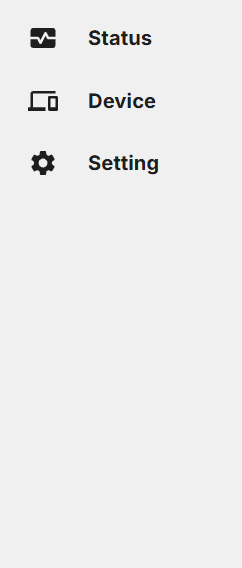
\includegraphics[width=0.3\textwidth]{pictures/Sidebar.png}
                \caption{Giao diện Sidebar}
                \label{fig:sidebar}
            \end{figure}
            \subsubsection{Import}
                \hspace*{0.6cm}Các thư viện và thành phần được nhập để xây dựng \texttt{Sidebar}:
                \begin{lstlisting}
    import React from 'react';
    import {
        Drawer, List, ListItem, ListItemIcon, ListItemText, Toolbar, Divider,
    } from '@mui/material';
    import StatusIcon from '@mui/icons-material/MonitorHeart';
    import DevicesIcon from '@mui/icons-material/Devices';
    import SettingIcon from '@mui/icons-material/Settings';
    import { Link, useLocation } from 'react-router-dom';
                \end{lstlisting}
                \begin{itemize}
                    \item \texttt{React}: Thư viện chính để xây dựng component.
                    \item \texttt{Material-UI}: Cung cấp các thành phần:
                    \begin{itemize}
                        \item \texttt{Drawer}: Thanh điều hướng bên.
                        \item \texttt{List}, \texttt{ListItem}, \texttt{ListItemIcon}, \texttt{ListItemText}: Tạo danh sách điều hướng.
                        \item \texttt{Toolbar}: Khoảng trống trên cùng để căn chỉnh với \texttt{AppBar}.
                        \item \texttt{Divider}: Đường phân cách.
                    \end{itemize}
                    \item \texttt{StatusIcon}, \texttt{DevicesIcon}, \texttt{SettingIcon}: Biểu tượng cho các mục điều hướng.
                    \item \texttt{Link}, \texttt{useLocation}: Từ \texttt{react-router-dom} để điều hướng và lấy đường dẫn hiện tại.
                \end{itemize}

            \subsubsection{Biến và Cấu Hình}
                \hspace*{0.6cm}Định nghĩa chiều rộng và danh sách mục điều hướng:
                \begin{lstlisting}
    const expandedWidth = 200;
    const collapsedWidth = 75;

    const menuItems = [
        { label: 'Status', path: '/status/', icon: <StatusIcon /> },
        { label: 'Device', path: '/device/', icon: <DevicesIcon /> },
        { label: 'Setting', path: '/setting/', icon: <SettingIcon /> },
    ];
                \end{lstlisting}
                \begin{itemize}
                    \item \texttt{expandedWidth}: Chiều rộng khi sidebar mở (200px).
                    \item \texttt{collapsedWidth}: Chiều rộng khi sidebar rút gọn (75px).
                    \item \texttt{menuItems}: Mảng chứa các mục điều hướng, mỗi mục có nhãn (\texttt{label}), đường dẫn (\texttt{path}), và biểu tượng (\texttt{icon}).
                \end{itemize}

            \subsubsection{Component Sidebar}
                \hspace*{0.6cm}Component nhận prop để điều khiển trạng thái mở/rút gọn:
                \begin{lstlisting}
    const Sidebar = ({ open }) => {
        const location = useLocation();
                \end{lstlisting}
                \begin{itemize}
                    \item \texttt{open}: Trạng thái mở (true) hoặc rút gọn (false) của sidebar.
                    \item \texttt{useLocation}: Hook lấy đường dẫn hiện tại để xác định mục được chọn.
                \end{itemize}

            \subsubsection{Cấu Trúc JSX}
                \hspace*{0.6cm}Giao diện của \texttt{Sidebar} được định nghĩa trong JSX:
                \begin{lstlisting}
return (
    <Drawer
        variant="permanent"
        sx={{
            width: open ? expandedWidth : collapsedWidth,
            flexShrink: 0,
            '& .MuiDrawer-paper': {
                width: open ? expandedWidth : collapsedWidth,
                transition: 'width 0.3s',
                overflowX: 'hidden',
                boxSizing: 'border-box',
                backgroundColor: (theme) => theme.palette.background.sidebar,
                color: (theme) => theme.palette.text.primary,
                borderRight: 'none',
            },
        }}
    >
        <Toolbar />
        <Divider />
        <List>
            {menuItems.map((item) => {
                const selected = location.pathname === item.path;

                return (
                    <ListItem
                        key={item.path}
                        button
                        component={Link}
                        to={item.path}
                        selected={selected}
                        sx={(theme) => ({
                            minHeight: 50,
                            px: 2,
                            py: 1,
                            justifyContent: open ? 'initial' : 'center',
                            color: theme.palette.text.primary,
                            '&:hover': {
                                backgroundColor:
                                    theme.palette.action.hover,
                            },
                            '&.Mui-selected': {
                                backgroundColor:
                                    theme.palette.action.selected,
                                color: theme.palette.text.primary,
                            },
                        })}
                    >
                        <ListItemIcon
                            sx={(theme) => ({
                                minWidth: 40,
                                mr: open ? 2 : 'auto',
                                justifyContent: 'center',
                                color: theme.palette.text.primary,
                            })}
                        >
                            {item.icon}
                        </ListItemIcon>
                        {open && <ListItemText primary={item.label} />}
                    </ListItem>
                );
            })}
        </List>
    </Drawer>
);
                \end{lstlisting}
                \begin{itemize}
                    \item \texttt{Drawer}: Thanh điều hướng cố định (\texttt{variant="permanent"}) với:
                    \begin{itemize}
                        \item Chiều rộng động dựa trên \texttt{open} (\texttt{expandedWidth} hoặc \texttt{collapsedWidth}).
                        \item Hiệu ứng chuyển đổi mượt mà (\texttt{transition: 'width 0.3s'}).
                        \item Màu nền từ \texttt{theme.palette.background.sidebar}.
                        \item Không có viền phải (\texttt{borderRight: 'none'}).
                    \end{itemize}
                    \item \texttt{Toolbar}: Khoảng trống trên cùng để căn chỉnh với \texttt{AppBar}.
                    \item \texttt{Divider}: Đường phân cách giữa \texttt{Toolbar} và danh sách.
                    \item \texttt{List}: Danh sách các mục điều hướng, lặp qua \texttt{menuItems} để tạo:
                    \begin{itemize}
                        \item \texttt{ListItem}: Mỗi mục là một nút liên kết (\texttt{component={Link}}) tới \texttt{item.path}.
                        \item \texttt{selected}: Đánh dấu mục đang chọn nếu \texttt{location.pathname} khớp \texttt{item.path}.
                        \item Tùy chỉnh giao diện: Căn giữa khi rút gọn, căn trái khi mở; hiệu ứng hover và chọn từ theme.
                    \end{itemize}
                    \item \texttt{ListItemIcon}: Hiển thị biểu tượng, căn giữa khi rút gọn.
                    \item \texttt{ListItemText}: Hiển thị nhãn khi \texttt{open} là \texttt{true}.
                \end{itemize}

            \subsubsection{Export}
                \hspace*{0.6cm}Component được xuất để sử dụng trong ứng dụng:
                \begin{lstlisting}
    export default Sidebar;
                \end{lstlisting}

            \subsubsection{Chức Năng Chính}
                \begin{itemize}
                    \item \textbf{Điều Hướng Ứng Dụng}: Cung cấp các mục điều hướng ("Status", "Device", "Setting") với liên kết tới các trang tương ứng thông qua \texttt{react-router-dom}.
                    \item \textbf{Trạng Thái Mở/Rút Gọn}: Hiển thị đầy đủ (với nhãn) hoặc rút gọn (chỉ biểu tượng) dựa trên prop \texttt{open}.
                    \item \textbf{Đánh Dấu Mục Được Chọn}: Tự động làm nổi bật mục tương ứng với đường dẫn hiện tại.
                    \item \textbf{Giao Diện}: Sử dụng Material-UI để tạo bố cục mượt mà, hiệu ứng chuyển đổi và giao diện tùy chỉnh theo theme.
                \end{itemize}
    \section{PAGES}
        \subsection{Status}
            \hspace*{0.6cm}Là trang hiển thị trạng thái của hệ thống, ử dụng \texttt{axios} để lấy danh sách thiết bị từ API và Socket.IO để nhận cập nhật trạng thái thiết bị thời gian thực. Nó hiển thị danh sách thiết bị với tên, trạng thái và thời gian cập nhật, đồng thời xử lý xác thực người dùng và thông báo lỗi qua \texttt{SnackbarContext}.
            \begin{figure}[H]
                \centering
                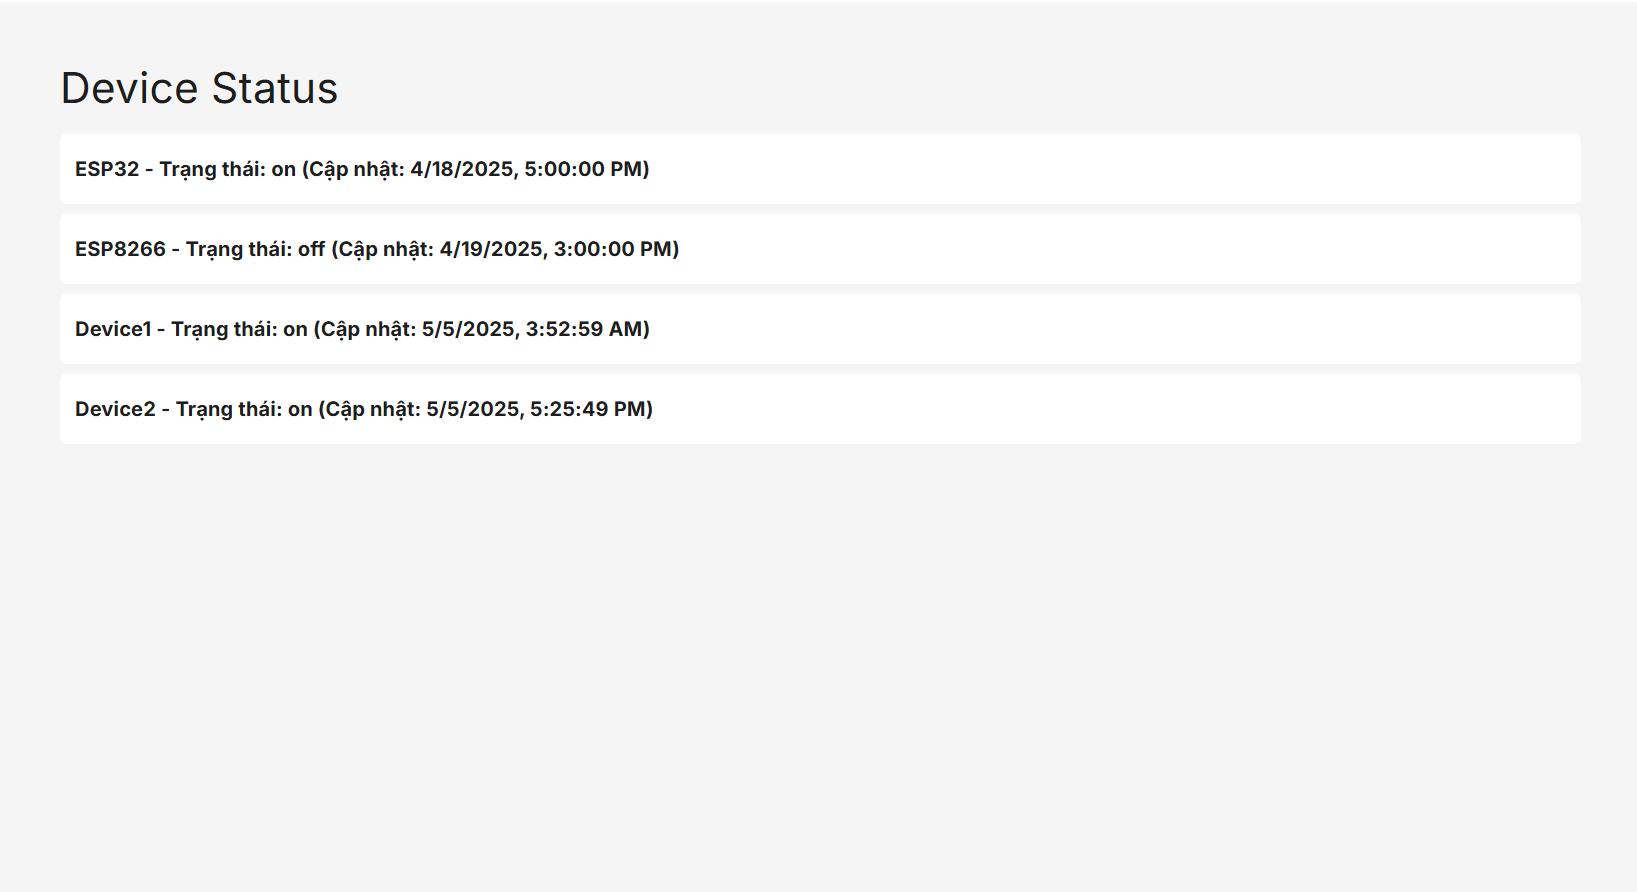
\includegraphics[width=1\textwidth]{pictures/Status.png}
                \caption{Giao diện Status}
                \label{fig:status}
            \end{figure}
            \subsubsection{Import}
                \hspace*{0.6cm}Các thư viện và thành phần được nhập:
                \begin{lstlisting}
    import { Box, Typography, List, ListItem, ListItemText } from "@mui/material";
    import { useTheme } from "@mui/material/styles";
    import React, { useEffect, useState } from "react";
    import axios from "axios";
    import io from "socket.io-client";
    import { useNavigate } from "react-router-dom";
    import { useSnackbar } from '../context/SnackbarContext';
                \end{lstlisting}
                \begin{itemize}
                    \item \texttt{Material-UI}: Cung cấp \texttt{Box}, \texttt{Typography}, \texttt{List}, \texttt{ListItem}, \texttt{ListItemText} cho giao diện và \texttt{useTheme} để lấy theme.
                    \item \texttt{React}, \texttt{useEffect}, \texttt{useState}: Quản lý trạng thái và vòng đời component.
                    \item \texttt{axios}: Gửi yêu cầu HTTP tới API.
                    \item \texttt{io}: Kết nối Socket.IO thời gian thực.
                    \item \texttt{useNavigate}: Điều hướng trang từ \texttt{react-router-dom}.
                    \item \texttt{useSnackbar}: Hook hiển thị thông báo từ \texttt{SnackbarContext}.
                \end{itemize}

            \subsubsection{API và Socket.IO}
                \hspace*{0.6cm}Định nghĩa URL API và kết nối Socket.IO:
                \begin{lstlisting}
    const API_URL = import.meta.env.VITE_API_URL || "http://localhost:5000";

    const getToken = () => {
        return document.cookie.split("; ").find(row => row.startsWith("authToken="))?.split("=")[1] || null;
    };

    const socket = io(API_URL, {
        reconnection: true,
        reconnectionAttempts: 5,
        reconnectionDelay: 1000,
        transports: ["websocket", "polling"],
        auth: { token: getToken() }
    });
                \end{lstlisting}
                \begin{itemize}
                    \item \texttt{API\_URL}: Lấy từ biến môi trường hoặc mặc định \texttt{http://localhost:5000}.
                    \item \texttt{getToken}: Lấy token xác thực từ cookie.
                    \item \texttt{socket}: Kết nối Socket.IO với:
                    \begin{itemize}
                        \item Tự động thử lại 5 lần, cách nhau 1 giây.
                        \item Ưu tiên WebSocket, fallback sang polling.
                        \item Gửi token xác thực qua \texttt{auth}.
                    \end{itemize}
                \end{itemize}

            \subsubsection{Component StatusPage}
                \hspace*{0.6cm}Component nhận prop \texttt{user}:
                \begin{lstlisting}
    const StatusPage = ({ user }) => {
                \end{lstlisting}
                \begin{itemize}
                    \item \texttt{user}: Thông tin người dùng để kiểm tra đăng nhập.
                \end{itemize}

            \subsubsection{Trạng Thái}
                \hspace*{0.6cm}Quản lý trạng thái:
                \begin{lstlisting}
    const theme = useTheme();
    const navigate = useNavigate();
    const [devices, setDevices] = useState([]);
    const [error, setError] = useState(null);
    const [loading, setLoading] = useState(true);
    const { showSnackbar } = useSnackbar();
                \end{lstlisting}
                \begin{itemize}
                    \item \texttt{theme}: Lấy theme từ Material-UI.
                    \item \texttt{navigate}: Hàm điều hướng trang.
                    \item \texttt{devices}: Danh sách thiết bị từ API.
                    \item \texttt{error}: Lưu thông báo lỗi.
                    \item \texttt{loading}: Trạng thái tải dữ liệu.
                    \item \texttt{showSnackbar}: Hiển thị thông báo.
                \end{itemize}

            \subsubsection{Xử Lý Dữ Liệu và Socket.IO}
                \hspace*{0.6cm}Sử dụng \texttt{useEffect} để lấy dữ liệu và thiết lập Socket.IO:
                \begin{lstlisting}
    useEffect(() => {
        if (!user) {
            navigate("/login");
            return;
        }

        const fetchDevices = async () => {
            try {
                console.log("Fetching devices from API:", `${API_URL}/api/devices`);
                const response = await axios.get(`${API_URL}/api/devices`, {
                    withCredentials: true,
                });
                console.log("Devices fetched:", response.data);
                setDevices(response.data);
                setLoading(false);
            } catch (error) {
                const errorMsg = error.response?.data?.message || error.message;
                console.error("Error fetching devices:", errorMsg);
                setError(`Error fetching devices: ${errorMsg}`);
                showSnackbar(`Error fetching devices: ${errorMsg}`, "error");
                setLoading(false);
                if (errorMsg.includes("") || errorMsg.includes("Invalid token")) {
                    navigate("/login");
                }
            }
        };
        fetchDevices();

        socket.on("connect", () => {
            console.log("Connected to Socket.IO from Frontend! ID:"", socket.id);
        });
        socket.on("deviceUpdate", (updatedDevice) => {
            console.log("Receive deviceUpdate:", updatedDevice);
            try {
                if (!updatedDevice || !updatedDevice.name) {
                    console.warn("Invalid deviceUpdate data", updatedDevice);
                    return;
                }
                setDevices((prev) => {
                    const existingDevice = prev.find((device) => device.name === updatedDevice.name);
                    if (existingDevice) {
                        return prev.map((device) =>
                            device.name === updatedDevice.name ? updatedDevice : device
                        );
                    }
                    return [...prev, updatedDevice];
                });
            } catch (error) {
                console.error("Error processing deviceUpdate:", error.message);
                setError(`Error processing deviceUpdate: ${error.message}`);
                showSnackbar(`Error processing deviceUpdate: ${error.message}`, "error");
            }
        });
        socket.on("connect_error", (err) => {
            console.error("Socket.IO connection error:", err.message);
            setError(`Socket.IO connection error: ${err.message}`);
            showSnackbar(`Socket.IO connection error: ${err.message}`, "error");
            navigate("/login");
        });

        return () => {
            socket.off("deviceUpdate");
            socket.off("connect");
            socket.off("connect_error");
            socket.disconnect();
        };
    }, [user, navigate]);
                \end{lstlisting}
                \begin{itemize}
                    \item Kiểm tra \texttt{user}: Nếu chưa đăng nhập, chuyển hướng tới \texttt{/login}.
                    \item \texttt{fetchDevices}: Gửi yêu cầu GET tới \texttt{/api/devices} để lấy danh sách thiết bị, xử lý lỗi và hiển thị thông báo qua \texttt{showSnackbar}.
                    \item Socket.IO:
                    \begin{itemize}
                        \item Lắng nghe \texttt{connect}: Ghi log khi kết nối thành công.
                        \item Lắng nghe \texttt{deviceUpdate}: Cập nhật hoặc thêm thiết bị vào \texttt{devices}.
                        \item Lắng nghe \texttt{connecterror}: Hiển thị lỗi và chuyển hướng tới \texttt{/login}.
                    \end{itemize}
                    \item Cleanup: Hủy các listener và ngắt kết nối Socket.IO khi component unmount.
                \end{itemize}

            \subsubsection{Cấu Trúc JSX}
                \hspace*{0.6cm}Giao diện của \texttt{StatusPage}:
                \begin{lstlisting}
return (
    <Box sx={{ p: 3, minHeight: "100vh", bgcolor: "background.default" }}>
        <Typography variant="h4" sx={{ color: "text.primary", mb: 2 }}>
            Device Status
        </Typography>
        {loading && (
        <Typography sx={{ color: "text.secondary" }}>
            Loading devices...
        </Typography>
        )}
        {error && (
        <Typography sx={{ color: "error.main" }}>
            {error}
        </Typography>
        )}
        {devices.length === 0 && !loading ? (
        <Typography sx={{ color: "text.secondary" }}>
            No devices found.
        </Typography>
        ) : (
            <List sx={{ p: 0 }}>
                {devices.map((device, index) => (
                    <ListItem
                        key={device.name || index}
                        sx={{
                            my: 1,
                            p: 1.5,
                            bgcolor: "background.paper",
                            borderRadius: "5px",
                            color: "text.primary"
                        }}
                    >
                        <ListItemText
                            primary={`${device.name} - Status: ${device.status} (Update: ${
                                device.updatedAt ? new Date(device.updatedAt).
                                toLocaleString() : "N/A"
                            })`}
                        />
                    </ListItem>
                ))}
            </List>
        )}  
    </Box>
);
                \end{lstlisting}
                \begin{itemize}
                    \item \texttt{Box}: Container chính với padding 3, chiều cao tối thiểu 100vh, màu nền từ theme.
                    \item \texttt{Typography} (tiêu đề): "Device Status" với kiểu \texttt{h4}.
                    \item Trạng thái tải: Hiển thị "Đang tải thiết bị..." khi \texttt{loading} là \texttt{true}.
                    \item Lỗi: Hiển thị thông báo lỗi với màu đỏ nếu \texttt{error} tồn tại.
                    \item Không có thiết bị: Hiển thị "Không có thiết bị nào" nếu \texttt{devices} rỗng và không tải.
                    \item Danh sách thiết bị: Sử dụng \texttt{List} và \texttt{ListItem} để hiển thị thông tin thiết bị (tên, trạng thái, thời gian cập nhật).
                \end{itemize}

            \subsubsection{Export}
                \hspace*{0.6cm}Component được xuất:
                \begin{lstlisting}
    export default StatusPage;
                \end{lstlisting}

            \subsubsection{Chức Năng Chính}
                \begin{itemize}
                    \item \textbf{Xác Thực Người Dùng}: Chuyển hướng tới \texttt{/login} nếu chưa đăng nhập hoặc token không hợp lệ.
                    \item \textbf{Lấy Danh Sách Thiết Bị}: Gửi yêu cầu API để lấy danh sách thiết bị ban đầu.
                    \item \textbf{Cập Nhật Thời Gian Thực}: Nhận cập nhật trạng thái thiết bị qua Socket.IO (\texttt{deviceUpdate}).
                    \item \textbf{Xử Lý Lỗi}: Hiển thị thông báo lỗi qua \texttt{showSnackbar} và chuyển hướng nếu cần.
                    \item \textbf{Giao Diện}: Hiển thị danh sách thiết bị với thông tin rõ ràng, hỗ trợ trạng thái tải và thông báo lỗi.
                \end{itemize}
        \subsection{Device}
            \hspace*{0.6cm}Là trang hiển thị danh sách thiết bị, cho phép người dùng thêm, sửa và xóa thiết bị. Nó sử dụng \texttt{axios} để gửi yêu cầu tới API và Socket.IO để nhận cập nhật thời gian thực. Giao diện bao gồm danh sách thiết bị, các nút hành động và hộp thoại xác nhận.
            \begin{figure}[H]
                \centering
                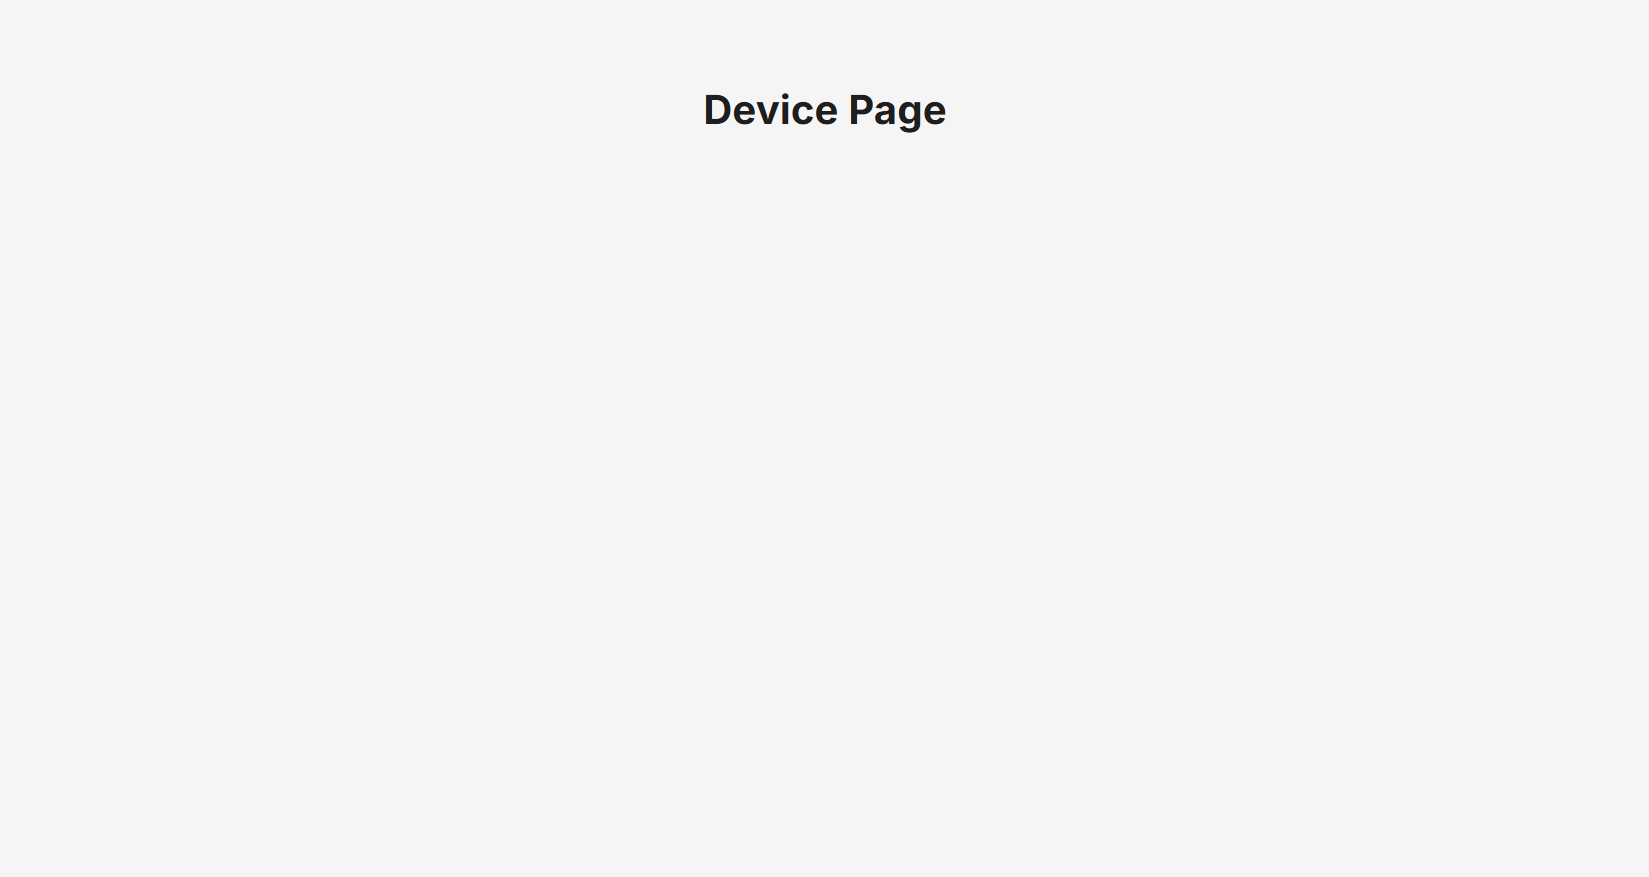
\includegraphics[width=1\textwidth]{pictures/Device.png}
                \caption{Giao diện Device}
                \label{fig:device}
            \end{figure}
        \subsection{Setting}
            \hspace*{0.6cm}Là trang sử dụng Material-UI để cung cấp giao diện cho phép người dùng thiết lập các tùy chỉnh của trang, đầu tiên là chuyển đổi giữa chế độ sáng (\texttt{light}) và chế độ tối (\texttt{dark}) thông qua một công tắc (\texttt{Switch})
            \begin{figure}[H]
                \centering
                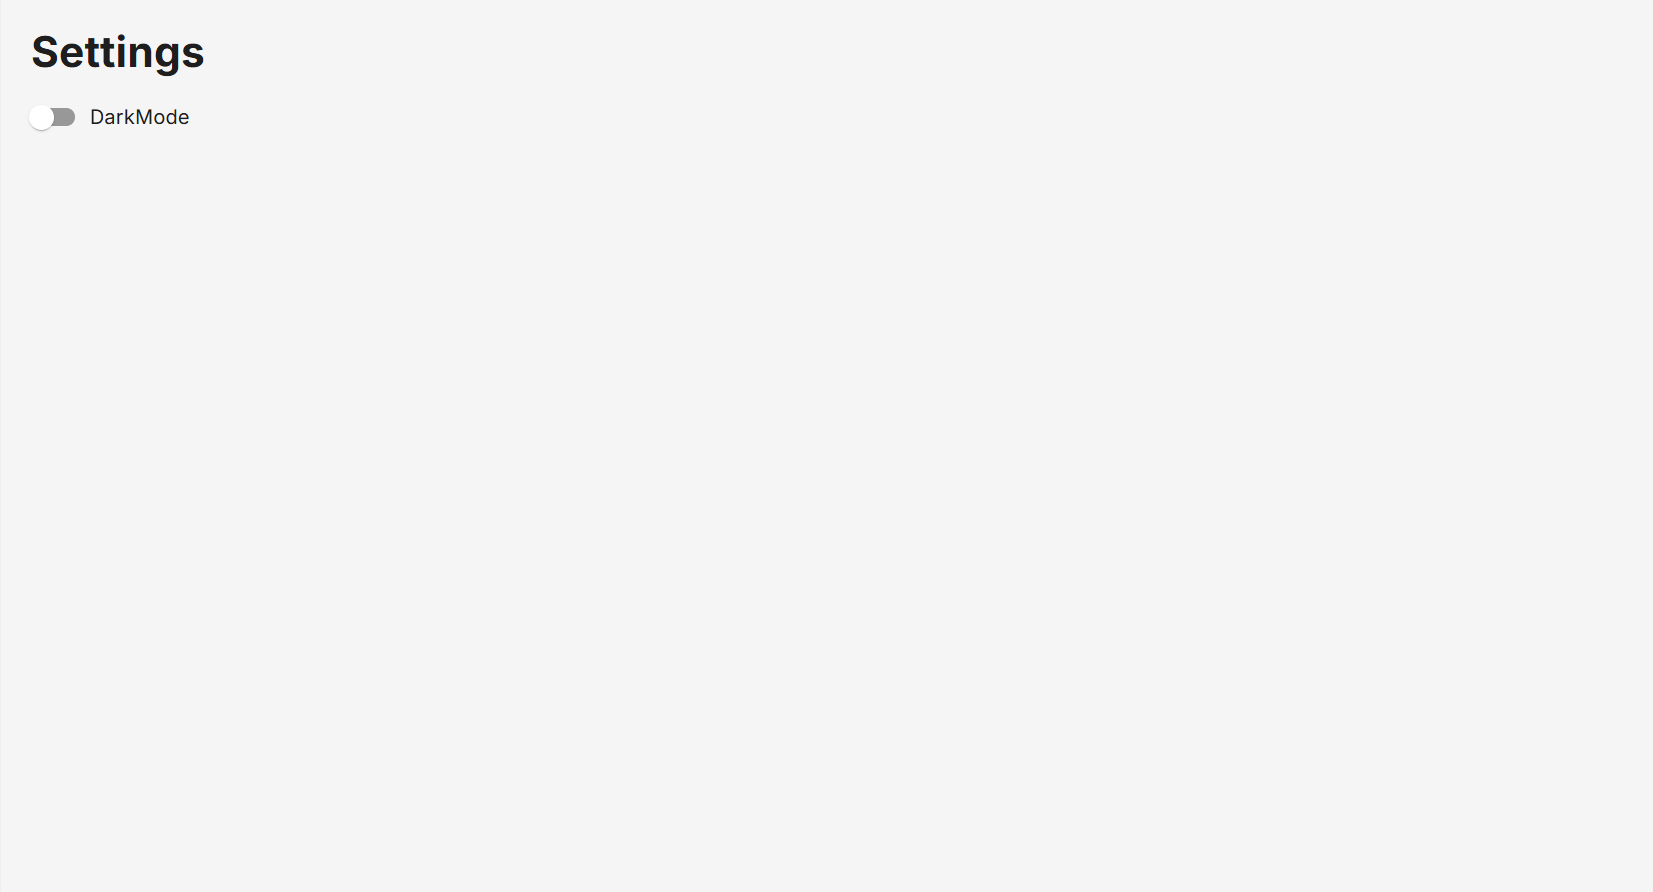
\includegraphics[width=1\textwidth]{pictures/Setting.png}
                \caption{Giao diện Setting}
                \label{fig:setting}
            \end{figure}
            \subsubsection{Import}
                \hspace{0.6cm}Các thư viện và thành phần được nhập:
                \begin{lstlisting}
                import React from 'react';
                import { Typography, Switch, FormControlLabel } from '@mui/material';
                \end{lstlisting}
                \begin{itemize}
                    \item \texttt{React}: Thư viện chính để xây dựng component.
                    \item \texttt{Material-UI}: Cung cấp các thành phần:
                    \begin{itemize}
                        \item \texttt{Typography}: Hiển thị tiêu đề.
                        \item \texttt{Switch}: Công tắc để chuyển đổi chế độ.
                        \item \texttt{FormControlLabel}: Nhãn cho công tắc.
                    \end{itemize}
                \end{itemize}

            \subsubsection{Component SettingPage}
                \hspace*{0.6cm}Component nhận các props:
                \begin{lstlisting}
                const SettingPage = ({ mode, setMode }) => {
                \end{lstlisting}
                \begin{itemize}
                    \item \texttt{mode}: Chế độ giao diện hiện tại (\texttt{light} hoặc \texttt{dark}).
                    \item \texttt{setMode}: Hàm cập nhật chế độ giao diện.
                \end{itemize}

            \subsubsection{Xử Lý Sự Kiện}
                \hspace*{0.6cm}Hàm xử lý chuyển đổi chế độ:
                \begin{lstlisting}
                const handleToggle = () => {
                    setMode(mode === 'light' ? 'dark' : 'light');
                };
                \end{lstlisting}
                \begin{itemize}
                    \item \texttt{handleToggle}: Chuyển đổi \texttt{mode} giữa \texttt{light} và \texttt{dark} bằng cách gọi \texttt{setMode}.
                \end{itemize}

            \subsubsection{Cấu Trúc JSX}
                \hspace*{0.6cm}Giao diện của \texttt{SettingPage}:
                \begin{lstlisting}
    return (
        <div>
            <Typography variant="h4" gutterBottom fontWeight="bold">
                Settings
            </Typography>

            <FormControlLabel
                control={<Switch checked={mode === 'dark'} onChange={handleToggle} />}
                label={mode === 'dark' ? 'LightMode' : 'DarkMode'}
            />
        </div>
    );
                \end{lstlisting}
                \begin{itemize}
                    \item \texttt{div}: Container chính cho giao diện.
                    \item \texttt{Typography}: Tiêu đề "Settings" với kiểu \texttt{h4}, in đậm, có khoảng cách dưới (\texttt{gutterBottom}).
                    \item \texttt{FormControlLabel}: Nhãn và công tắc:
                    \begin{itemize}
                        \item \texttt{control}: \texttt{Switch} được chọn khi \texttt{mode} là \texttt{dark}, gọi \texttt{handleToggle} khi thay đổi.
                        \item \texttt{label}: Hiển thị \texttt{LightMode} khi \texttt{mode} là \texttt{dark}, và \texttt{DarkMode} khi \texttt{mode} là \texttt{light}.
                    \end{itemize}
                \end{itemize}

            \subsubsection{Export}
                \hspace*{0.6cm}Component được xuất:
                \begin{lstlisting}
    export default SettingPage;
                \end{lstlisting}

            \subsubsection{Chức Năng Chính}
                \begin{itemize}
                    \item \textbf{Chuyển Đổi Chế Độ Giao Diện}: Cho phép người dùng chuyển đổi giữa chế độ sáng (\texttt{light}) và chế độ tối (\texttt{dark}) thông qua công tắc.
                    \item \textbf{Giao Diện Trực Quan}: Sử dụng Material-UI để tạo bố cục đơn giản với tiêu đề và công tắc được sắp xếp rõ ràng.
                    \item \textbf{Quản Lý Trạng Thái}: Nhận và cập nhật trạng thái \texttt{mode} thông qua props \texttt{mode} và \texttt{setMode}.
                \end{itemize}
    \section{CONTEXTS}
        \subsection{SnackbarContext}
            \hspace*{0.6cm}Dùng đề hiển thị các thông báo của ứng dụng sử dụng Snackbar trong MUI thay cho thông báo mặc định dùng Alert của Javascript.
            \begin{figure}[H]
                \centering
                
\includegraphics[width=0.5\textwidth]{pictures/Snackbar.png}
                \caption{Giao diện Snackbar}
                \label{fig:snackbar}
            \end{figure}
            \subsubsection{Import}
                \hspace*{0.6cm}Các thư viện và thành phần được nhập:
                \begin{lstlisting}
    import React, { createContext, useContext, useState } from 'react';
    import { Snackbar, Alert, Slide } from '@mui/material';
                \end{lstlisting}
                \begin{itemize}
                    \item \texttt{React}, \texttt{createContext}, \texttt{useContext}, \texttt{useState}: Quản lý ngữ cảnh và trạng thái.
                    \item \texttt{Material-UI}: Cung cấp:
                    \begin{itemize}
                        \item \texttt{Snackbar}: Hiển thị thông báo tạm thời.
                        \item \texttt{Alert}: Thành phần thông báo với mức độ nghiêm trọng.
                        \item \texttt{Slide}: Hiệu ứng trượt cho thông báo.
                    \end{itemize}
                \end{itemize}

            \subsubsection{Tạo Context}
                \hspace*{0.6cm}Tạo ngữ cảnh để chia sẻ hàm \texttt{showSnackbar}:
                \begin{lstlisting}
    const SnackbarContext = createContext();
                \end{lstlisting}
                \begin{itemize}
                    \item \texttt{SnackbarContext}: Ngữ cảnh để các component con truy cập \texttt{showSnackbar}.
                \end{itemize}

            \subsubsection{Component SnackbarProvider}
                \hspace*{0.6cm}Component cung cấp ngữ cảnh và giao diện thông báo:
                \begin{lstlisting}
    export const SnackbarProvider = ({ children }) => {
        const [open, setOpen] = useState(false);
        const [message, setMessage] = useState('');
        const [severity, setSeverity] = useState('success');
                \end{lstlisting}
                \begin{itemize}
                    \item \texttt{children}: Các component con được bao bọc bởi \texttt{SnackbarProvider}.
                    \item \texttt{open}: Trạng thái hiển thị của snackbar (\texttt{true}/\texttt{false}).
                    \item \texttt{message}: Nội dung thông báo.
                    \item \texttt{severity}: Mức độ nghiêm trọng (\texttt{success}, \texttt{error}, v.v.).
                \end{itemize}

            \subsubsection{Xử Lý Thông Báo}
                \hspace*{0.6cm}Hàm kích hoạt và đóng thông báo:
                \begin{lstlisting}
    const showSnackbar = (msg, sev = 'success') => {
        setMessage(msg);
        setSeverity(sev);
        setOpen(true);
    };

    const handleClose = (event, reason) => {
        if (reason === 'clickaway') {
            return;
        }
        setOpen(false);
    };
                \end{lstlisting}
                \begin{itemize}
                    \item \texttt{showSnackbar}: Cập nhật \texttt{message}, \texttt{severity} và mở snackbar.
                    \item \texttt{handleClose}: Đóng snackbar, bỏ qua nếu người dùng click ra ngoài (\texttt{clickaway}).
                \end{itemize}

            \subsubsection{Cấu Trúc JSX}
                \hspace*{0.6cm}Giao diện và cung cấp ngữ cảnh:
                \begin{lstlisting}
return (
    <SnackbarContext.Provider value={{ showSnackbar }}>
        {children}
        <Snackbar
            open={open}
            autoHideDuration={3000}
            onClose={handleClose}
            anchorOrigin={{ vertical: 'top', horizontal: 'right' }}
            TransitionComponent={Slide}
            transitionDuration={500}
        >
            <Alert
                onClose={handleClose}
                severity={severity}
                sx={{
                    width: '100%',
                    bgcolor: severity === 'success' ? '#4caf50' : '#f44336',
                    color: '#fff',
                    '& .MuiAlert-icon': {
                        color: '#fff',
                    },
                    borderRadius: '8px',
                    boxShadow: '0px 4px 12px rgba(0, 0, 0, 0.1)',
                }}
            >
                {message}
            </Alert>
        </Snackbar>
    </SnackbarContext.Provider>
);
                \end{lstlisting}
                \begin{itemize}
                    \item \texttt{SnackbarContext.Provider}: Cung cấp \texttt{showSnackbar} cho các component con.
                    \item \texttt{children}: Hiển thị các component con.
                    \item \texttt{Snackbar}: Thông báo với:
                    \begin{itemize}
                        \item Hiển thị khi \texttt{open} là \texttt{true}.
                        \item Tự động ẩn sau 3 giây (\texttt{autoHideDuration={3000}}).
                        \item Vị trí góc trên bên phải (\texttt{anchorOrigin}).
                        \item Hiệu ứng trượt (\texttt{Slide}) trong 500ms.
                    \end{itemize}
                    \item \texttt{Alert}: Thành phần thông báo với:
                    \begin{itemize}
                        \item Mức độ \texttt{severity} (ảnh hưởng màu sắc).
                        \item Tùy chỉnh giao diện: Màu nền xanh (\texttt{\#4caf50}) cho \texttt{success}, đỏ (\texttt{\#f44336}) cho \texttt{error}; chữ và icon trắng; bo góc và bóng.
                    \end{itemize}
                \end{itemize}

            \subsubsection{Hook useSnackbar}
                \hspace*{0.6cm}Hook để truy cập \texttt{showSnackbar}:
                \begin{lstlisting}
    export const useSnackbar = () => {
        const context = useContext(SnackbarContext);
        if (!context) {
            throw new Error('useSnackbar must be used within a SnackbarProvider');
        }
        return context;
    };
                \end{lstlisting}
                \begin{itemize}
                    \item \texttt{useSnackbar}: Truy cập \texttt{SnackbarContext}, ném lỗi nếu không nằm trong \texttt{SnackbarProvider}.
                \end{itemize}

            \subsubsection{Chức Năng Chính}
                \begin{itemize}
                    \item \textbf{Hiển Thị Thông Báo}: Cho phép các component con kích hoạt thông báo với nội dung và mức độ nghiêm trọng tùy chỉnh qua \texttt{showSnackbar}.
                    \item \textbf{Hiệu Ứng Trượt}: Sử dụng \texttt{Slide} để tạo hiệu ứng mượt mà khi thông báo xuất hiện/biến mất.
                    \item \textbf{Tùy Chỉnh Giao Diện}: Tùy chỉnh màu sắc, bo góc và bóng cho thông báo dựa trên \texttt{severity}.
                    \item \textbf{Quản Lý Trạng Thái}: Điều khiển hiển thị, nội dung và loại thông báo thông qua trạng thái \texttt{open}, \texttt{message}, \texttt{severity}.
                \end{itemize}
    \section{HOOKS}
        \subsection{useAuth}
            \hspace*{0.6cm}Là một hook tùy chỉnh, cung cấp các chức năng quản lý xác thực người dùng, bao gồm đăng nhập và đăng xuất. Nó tích hợp với API thông qua \texttt{axios}, sử dụng Socket.IO để quản lý kết nối thời gian thực, và hiển thị thông báo qua \texttt{SnackbarContext}. Hook này được sử dụng trong các component như \texttt{Header} để xử lý trạng thái đăng nhập.
            \subsubsection{Import}
                \hspace*{0.6cm}Các thư viện và thành phần được nhập:
                \begin{lstlisting}
    import { useState } from "react";
    import { useNavigate } from "react-router-dom";
    import axios from "axios";
    import loginUser from "../api/loginUser";
    import { useSnackbar } from '../context/SnackbarContext';
                \end{lstlisting}
                \begin{itemize}
                    \item \texttt{useState}: Quản lý trạng thái cục bộ.
                    \item \texttt{useNavigate}: Điều hướng trang từ \texttt{react-router-dom}.
                    \item \texttt{axios}: Gửi yêu cầu HTTP tới API.
                    \item \texttt{loginUser}: Hàm API tùy chỉnh để đăng nhập.
                    \item \texttt{useSnackbar}: Hook hiển thị thông báo từ \texttt{SnackbarContext}.
                \end{itemize}

            \subsubsection{Hook useAuth}
                \hspace*{0.6cm}Hook nhận các tham số và quản lý trạng thái:
                \begin{lstlisting}
    const useAuth = (setUser, socket) => {
        const [email, setEmail] = useState("");
        const [password, setPassword] = useState("");
        const [openLogin, setOpenLogin] = useState(false);
        const { showSnackbar } = useSnackbar();
        const navigate = useNavigate();
                \end{lstlisting}
                \begin{itemize}
                    \item \texttt{setUser}: Hàm cập nhật trạng thái người dùng.
                    \item \texttt{socket}: Đối tượng Socket.IO để quản lý kết nối.
                    \item \texttt{email}, \texttt{setEmail}: Quản lý email nhập vào.
                    \item \texttt{password}, \texttt{setPassword}: Quản lý mật khẩu nhập vào.
                    \item \texttt{openLogin}, \texttt{setOpenLogin}: Điều khiển hiển thị hộp thoại đăng nhập.
                    \item \texttt{showSnackbar}: Hiển thị thông báo.
                    \item \texttt{navigate}: Điều hướng trang.
                \end{itemize}

            \subsubsection{Xử Lý Đăng Nhập}
                \hspace*{0.6cm}Hàm xử lý đăng nhập:
                \begin{lstlisting}
    const handleLogin = async () => {
        const res = await loginUser(email, password);
        if (res.success) {
            setUser({ username: res.username, avatar: res.avatar });
            localStorage.setItem("user", JSON.stringify({ username: res.username, avatar: res.avatar }));
            setOpenLogin(false);
            setPassword("");
            socket.connect();
            showSnackbar("Login successful", "success");
            navigate("/status");
        } else {
            showSnackbar(res.message || "Login failed", "error");
        }
    };
                \end{lstlisting}
                \begin{itemize}
                    \item Gọi \texttt{loginUser} với \texttt{email} và \texttt{password}.
                    \item Nếu thành công:
                    \begin{itemize}
                        \item Cập nhật \texttt{user} với \texttt{username} và \texttt{avatar}.
                        \item Lưu thông tin vào \texttt{localStorage}.
                        \item Đóng hộp thoại, xóa mật khẩu, kết nối Socket.IO.
                        \item Hiển thị thông báo thành công và chuyển hướng tới \texttt{/status}.
                    \end{itemize}
                    \item Nếu thất bại: Hiển thị thông báo lỗi.
                \end{itemize}

            \subsubsection{Xử Lý Đăng Xuất}
                \hspace*{0.6cm}Hàm xử lý đăng xuất:
                \begin{lstlisting}
    const handleLogout = async () => {
        try {
            await axios.post(
                `${import.meta.env.VITE_API_URL}/api/users/logout`,
                {},
                { withCredentials: true }
            );
            setUser(null);
            localStorage.removeItem("user");
            socket.disconnect();
            showSnackbar("Logout successful", "success");
            navigate("/status");
        } catch (error) {
            console.error("Error during logout:", error);
            showSnackbar("Error during logout", "error");
        }
    };
                \end{lstlisting}
                \begin{itemize}
                    \item Gửi yêu cầu POST tới \texttt{/api/users/logout}.
                    \item Nếu thành công:
                    \begin{itemize}
                        \item Xóa \texttt{user} và \texttt{localStorage}.
                        \item Ngắt kết nối Socket.IO.
                        \item Hiển thị thông báo thành công và chuyển hướng tới \texttt{/status}.
                    \end{itemize}
                    \item Nếu thất bại: Ghi log và hiển thị thông báo lỗi.
                \end{itemize}

            \subsubsection{Trả Về}
                \hspace*{0.6cm}Hook trả về các giá trị và hàm:
                \begin{lstlisting}
    return {
        email,
        setEmail,
        password,
        setPassword,
        openLogin,
        setOpenLogin,
        handleLogin,
        handleLogout,
    };
                \end{lstlisting}
                \begin{itemize}
                    \item Trả về trạng thái (\texttt{email}, \texttt{password}, \texttt{openLogin}) và các hàm xử lý để sử dụng trong component.
                \end{itemize}

            \subsubsection{Export}
                \hspace*{0.6cm}Hook được xuất:
                \begin{lstlisting}
    export default useAuth;
                \end{lstlisting}

            \subsubsection{Chức Năng Chính}
                \begin{itemize}
                    \item \textbf{Quản Lý Đăng Nhập}: Xử lý đăng nhập thông qua API, cập nhật trạng thái người dùng, lưu trữ cục bộ, và kết nối Socket.IO.
                    \item \textbf{Quản Lý Đăng Xuất}: Gửi yêu cầu đăng xuất, xóa dữ liệu người dùng, ngắt Socket.IO, và điều hướng trang.
                    \item \textbf{Hiển Thị Thông Báo}: Sử dụng \texttt{showSnackbar} để thông báo kết quả đăng nhập/đăng xuất.
                    \item \textbf{Điều Hướng Trang}: Chuyển hướng tới \texttt{/status} sau khi đăng nhập hoặc đăng xuất.
                    \item \textbf{Quản Lý Trạng Thái}: Cung cấp trạng thái và hàm để điều khiển giao diện đăng nhập.
                \end{itemize}
    \section{API}
        \subsection{loginUser}
            \hspace*{0.6cm}Là một hàm API sử dụng \texttt{axios} để gửi yêu cầu đăng nhập người dùng tới server. Hàm này nhận email và mật khẩu, gửi yêu cầu POST tới endpoint API, và trả về thông tin người dùng nếu thành công hoặc thông báo lỗi nếu thất bại. Nó được sử dụng trong hook \texttt{useAuth} để xử lý logic đăng nhập.
            \subsection{Import}
                \hspace*{0.6cm}Thư viện được nhập:
                \begin{lstlisting}
    import axios from "axios";
                \end{lstlisting}
                \begin{itemize}
                    \item \texttt{axios}: Thư viện để gửi yêu cầu HTTP tới API.
                \end{itemize}

            \subsubsection{Cấu Hình Axios}
                \hspace*{0.6cm}Cấu hình mặc định cho \texttt{axios}:
                \begin{lstlisting}
    axios.defaults.withCredentials = true;
                \end{lstlisting}
                \begin{itemize}
                    \item \texttt{withCredentials}: Cho phép gửi cookie trong các yêu cầu HTTP, cần thiết cho xác thực dựa trên cookie.
                \end{itemize}

            \subsubsection{Hàm loginUser}
                \hspace*{0.6cm}Hàm xử lý đăng nhập:
                \begin{lstlisting}
    const loginUser = async (email, password) => {
        try {
            localStorage.removeItem("token");
            localStorage.removeItem("authToken");

            const res = await axios.post(`${import.meta.env.VITE_API_URL}/api/users/login`, {
                email,
                password,
            });
            localStorage.setItem("user", JSON.stringify({ username: res.data.username, avatar: res.data.avatar }));
            return { success: true, username: res.data.username, avatar: res.data.avatar };
        } catch (err) {
            return { success: false, message: err.response?.data?.message || "Login error" };
        }
    };
                \end{lstlisting}
                \begin{itemize}
                    \item \texttt{email}, \texttt{password}: Tham số đầu vào cho yêu cầu đăng nhập.
                    \item Xóa \texttt{token} và \texttt{authToken} từ \texttt{localStorage} để đảm bảo không sử dụng token cũ.
                    \item Gửi yêu cầu POST tới \texttt{/api/users/login} với \texttt{email} và \texttt{password}.
                    \item Nếu thành công:
                    \begin{itemize}
                        \item Lưu thông tin người dùng (\texttt{username}, \texttt{avatar}) vào \texttt{localStorage}.
                        \item Trả về đối tượng \texttt{\{ success: true, username, avatar \}}.
                    \end{itemize}
                    \item Nếu thất bại:
                    \begin{itemize}
                        \item Trả về đối tượng \texttt{\{ success: false, message \}} với thông báo lỗi từ server hoặc mặc định là \texttt{"Login error"}.
                    \end{itemize}
                \end{itemize}

            \subsubsection{Export}
                \hspace*{0.6cm}Hàm được xuất:
                \begin{lstlisting}
    export default loginUser;
                \end{lstlisting}

            \subsubsection{Chức Năng Chính}
                \begin{itemize}
                    \item \textbf{Gửi Yêu Cầu Đăng Nhập}: Sử dụng \texttt{axios} để gửi email và mật khẩu tới endpoint \texttt{/api/users/login}.
                    \item \textbf{Xử Lý Phản Hồi}: Lưu thông tin người dùng vào \texttt{localStorage} nếu thành công, hoặc trả về thông báo lỗi nếu thất bại.
                    \item \textbf{Xóa Token Cũ}: Xóa các token cũ từ \texttt{localStorage} trước khi đăng nhập để tránh xung đột.
                    \item \textbf{Hỗ Trợ Xác Thực Cookie}: Cấu hình \texttt{withCredentials} cho phép gửi cookie xác thực.
                \end{itemize}
    \section{APP}
        \hspace*{0.6cm}Là thành phần chính của ứng dụng, chịu trách nhiệm tổ chức giao diện, quản lý trạng thái toàn cục (người dùng, chế độ giao diện, sidebar), và định tuyến các trang. Nó tích hợp Material-UI để tạo giao diện, \texttt{react-router-dom} cho định tuyến, và \texttt{SnackbarProvider} cho thông báo đồng thời cũng kiểm tra xác thực người dùng khi khởi động.
        \subsection{Import}
            \hspace*{0.6cm}Các thư viện và thành phần được nhập:
            \begin{lstlisting}
    import React, { useState, useEffect } from 'react';
    import { Routes, Route, Navigate } from 'react-router-dom';
    import { Box, Toolbar, CssBaseline, ThemeProvider } from '@mui/material';
    import { getTheme } from './theme';
    import Header from './components/Header';
    import Sidebar from './components/Sidebar';
    import StatusPage from './pages/StatusPage';
    import DevicePage from './pages/DevicePage';
    import SettingPage from './pages/SettingPage';
    import { SnackbarProvider } from './context/SnackbarContext';
    import axios from 'axios';
            \end{lstlisting}
            \begin{itemize}
                \item \texttt{React}, \texttt{useState}, \texttt{useEffect}: Quản lý trạng thái và vòng đời component.
                \item \texttt{react-router-dom}: \texttt{Routes}, \texttt{Route}, \texttt{Navigate} cho định tuyến.
                \item \texttt{Material-UI}: \texttt{Box}, \texttt{Toolbar}, \texttt{CssBaseline}, \texttt{ThemeProvider} cho giao diện và theme.
                \item \texttt{getTheme}: Hàm tùy chỉnh để tạo theme dựa trên chế độ sáng/tối.
                \item \texttt{Header}, \texttt{Sidebar}, \texttt{StatusPage}, \texttt{DevicePage}, \texttt{SettingPage}: Các component con.
                \item \texttt{SnackbarProvider}: Cung cấp ngữ cảnh thông báo.
                \item \texttt{axios}: Gửi yêu cầu HTTP tới API.
            \end{itemize}

        \subsection{API URL}
            \hspace*{0.6cm}Định nghĩa URL API:
            \begin{lstlisting}
            const API_URL = import.meta.env.VITE_API_URL || "http://localhost:5000";
            \end{lstlisting}
            \begin{itemize}
                \item \texttt{API\_URL}: Lấy từ biến môi trường hoặc mặc định \texttt{http://localhost:5000}.
            \end{itemize}

        \subsection{Component App}
            \hspace*{0.6cm}Component quản lý trạng thái toàn cục:
            \begin{lstlisting}
    const App = () => {
        const [sidebarOpen, setSidebarOpen] = useState(true);
        const [mode, setMode] = useState('light');
        const [user, setUser] = useState(() => {
            const savedUser = localStorage.getItem('user');
            return savedUser ? JSON.parse(savedUser) : null;
        });
        const [openLogin, setOpenLogin] = useState(false);
            \end{lstlisting}
            \begin{itemize}
                \item \texttt{sidebarOpen}: Trạng thái mở/rút gọn của sidebar.
                \item \texttt{mode}: Chế độ giao diện (\texttt{light} hoặc \texttt{dark}).
                \item \texttt{user}: Thông tin người dùng, khởi tạo từ \texttt{localStorage} hoặc \texttt{null}.
                \item \texttt{openLogin}: Điều khiển hiển thị hộp thoại đăng nhập.
            \end{itemize}

        \subsection{Kiểm Tra Xác Thực}
            \hspace*{0.6cm}Sử dụng \texttt{useEffect} để kiểm tra token:
            \begin{lstlisting}
    useEffect(() => {
        const verifyToken = async () => {
            try {
                const response = await axios.get(`${API_URL}/api/users/verify-token`, {
                    withCredentials: true,
                });
                if (!response.data.valid) {
                    setUser(null);
                    localStorage.removeItem('user');
                }
            } catch (error) {
                console.error("Error verifying token:", error);
                setUser(null);
                localStorage.removeItem('user');
            }
        };

        if (user) {
            verifyToken();
        }
    }, []);
            \end{lstlisting}
            \begin{itemize}
                \item Gửi yêu cầu GET tới \texttt{/api/users/verify-token} để kiểm tra token.
                \item Nếu token không hợp lệ hoặc có lỗi, xóa \texttt{user} và \texttt{localStorage}.
                \item Chỉ chạy khi có \texttt{user}, với mảng phụ thuộc rỗng (\texttt{[]}) để chạy một lần khi mount.
            \end{itemize}

        \subsection{Cấu Trúc JSX}
            \hspace*{0.6cm}Giao diện và định tuyến của ứng dụng:
            \begin{lstlisting}
return (
    <ThemeProvider theme={getTheme(mode)}>
        <SnackbarProvider>
            <CssBaseline />
            <Box sx={{ display: 'flex' }}>
                <Sidebar open={sidebarOpen} />
                <Box component="main" sx={{ flexGrow: 1, minHeight: '100vh' }}>
                    <Header
                        onToggleSidebar={() => setSidebarOpen(prev => !prev)}
                        user={user}
                        setUser={setUser}
                        openLogin={openLogin}
                        setOpenLogin={setOpenLogin}
                    />
                    <Toolbar />
                    <Box sx={{ p: 3 }}>
                        <Routes>
                            <Route
                                path="/status"
                                element={user ? <StatusPage user={user} /> : <Navigate to="/" />}
                            />
                            <Route
                                path="/device"
                                element={user ? <DevicePage user={user} /> : <Navigate to="/" />}
                            />
                            <Route
                                path="/setting"
                                element={<SettingPage mode={mode} setMode={setMode} />}
                            />
                            <Route path="/" element={<Navigate to="/status" />} />
                            <Route path="*" element={<Navigate to="/status" />} />
                        </Routes>
                    </Box>
                </Box>
            </Box>
        </SnackbarProvider>
    </ThemeProvider>
);
            \end{lstlisting}
            \begin{itemize}
                \item \texttt{ThemeProvider}: Áp dụng theme từ \texttt{getTheme(mode)}.
                \item \texttt{SnackbarProvider}: Bao bọc ứng dụng để cung cấp ngữ cảnh thông báo.
                \item \texttt{CssBaseline}: Đặt lại kiểu CSS mặc định của Material-UI.
                \item \texttt{Box} (container chính): Sử dụng flexbox để sắp xếp \texttt{Sidebar} và nội dung chính.
                \item \texttt{Sidebar}: Thanh điều hướng bên, điều khiển bởi \texttt{sidebarOpen}.
                \item \texttt{Box} (nội dung chính): Chứa \texttt{Header}, \texttt{Toolbar} (khoảng trống), và các trang.
                \item \texttt{Header}: Thanh điều hướng trên, truyền các prop để quản lý sidebar và người dùng.
                \item \texttt{Routes}: Định tuyến các trang:
                \begin{itemize}
                    \item \texttt{/status}: Hiển thị \texttt{StatusPage} nếu có \texttt{user}, ngược lại chuyển hướng tới \texttt{/}.
                    \item \texttt{/device}: Hiển thị \texttt{DevicePage} nếu có \texttt{user}, ngược lại chuyển hướng tới \texttt{/}.
                    \item \texttt{/setting}: Hiển thị \texttt{SettingPage} để chuyển đổi chế độ sáng/tối.
                    \item \texttt{/} và \texttt{*}: Chuyển hướng tới \texttt{/status}.
                \end{itemize}
            \end{itemize}

        \subsection{Export}
            \hspace*{0.6cm}Component được xuất:
            \begin{lstlisting}
    export default App;
            \end{lstlisting}

        \subsection{Chức Năng Chính}
            \begin{itemize}
                \item \textbf{Quản Lý Giao Diện}: Sử dụng Material-UI để tổ chức bố cục với sidebar, header và nội dung chính, hỗ trợ chế độ sáng/tối qua \texttt{mode}.
                \item \textbf{Xác Thực Người Dùng}: Kiểm tra token khi khởi động, tự động đăng xuất nếu token không hợp lệ.
                \item \textbf{Định Tuyến Trang}: Sử dụng \texttt{react-router-dom} để điều hướng giữa các trang \texttt{StatusPage}, \texttt{DevicePage}, \texttt{SettingPage}, với bảo vệ tuyến đường dựa trên trạng thái \texttt{user}.
                \item \textbf{Quản Lý Trạng Thái Toàn Cục}: Quản lý \texttt{user}, \texttt{sidebarOpen}, \texttt{mode}, và \texttt{openLogin}.
                \item \textbf{Hiển Thị Thông Báo}: Tích hợp \texttt{SnackbarProvider} để hiển thị thông báo trong toàn ứng dụng.
            \end{itemize}

                

           
                
                
    
                            
    \chapter{BACK END}
    \section{Cấu trúc hệ thống}
        \subsection{Mô hình Client - Server}
            \begin{figure}[H]
                \centering
                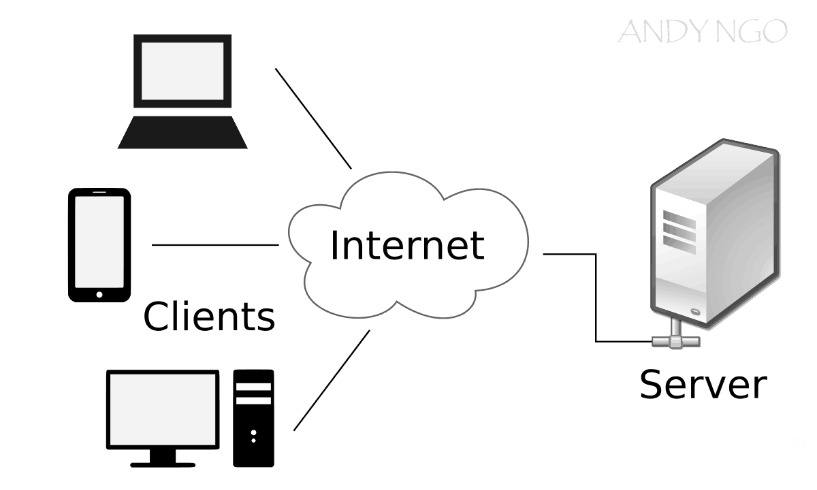
\includegraphics[width=0.8\textwidth]{pictures/ServerClient.png}
                \caption{Mô hình Client - Server}
                \label{fig:client-server}
            \end{figure}
            \hspace*{0.6cm}Mô hình Client - Server là một mô hình kiến trúc mạng trong đó các ứng dụng được chia thành hai phần: client và server. Client là phần mềm chạy trên máy tính của người dùng, trong khi server là phần mềm chạy trên máy chủ. Client gửi yêu cầu đến server và nhận phản hồi từ server.
        \subsection{Kiến trúc RESTful API}
            \hspace*{0.6cm}Kiến trúc RESTful API là một kiểu kiến trúc phần mềm cho phép các ứng dụng giao tiếp với nhau thông qua HTTP. RESTful API sử dụng các phương thức HTTP như GET, POST, PUT, DELETE để thực hiện các thao tác CRUD (Create, Read, Update, Delete) trên tài nguyên.
            \begin{figure}[H]
                \centering
                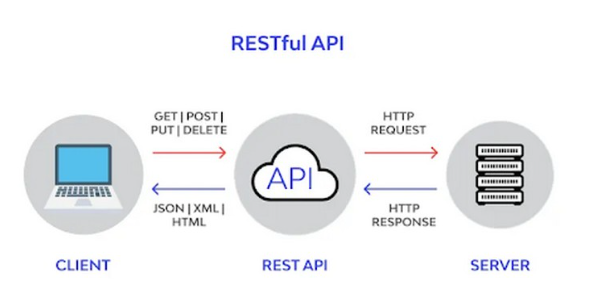
\includegraphics[width=0.8\textwidth]{pictures/RESTfulAPI.png}
                \caption{Kiến trúc RESTful API}
                \label{fig:restful-api}
            \end{figure}
        \subsection{Mô hình MVC}
            \hspace*{0.6cm}Mô hình MVC (Model-View-Controller) là một mô hình thiết kế phần mềm được sử dụng phổ biến trong phát triển ứng dụng web. Mô hình này chia ứng dụng thành ba phần: Model (mô hình), View (giao diện) và Controller (bộ điều khiển). Mỗi phần có nhiệm vụ riêng và tương tác với nhau để tạo ra ứng dụng hoàn chỉnh.
            \begin{figure}[H]
                \centering
                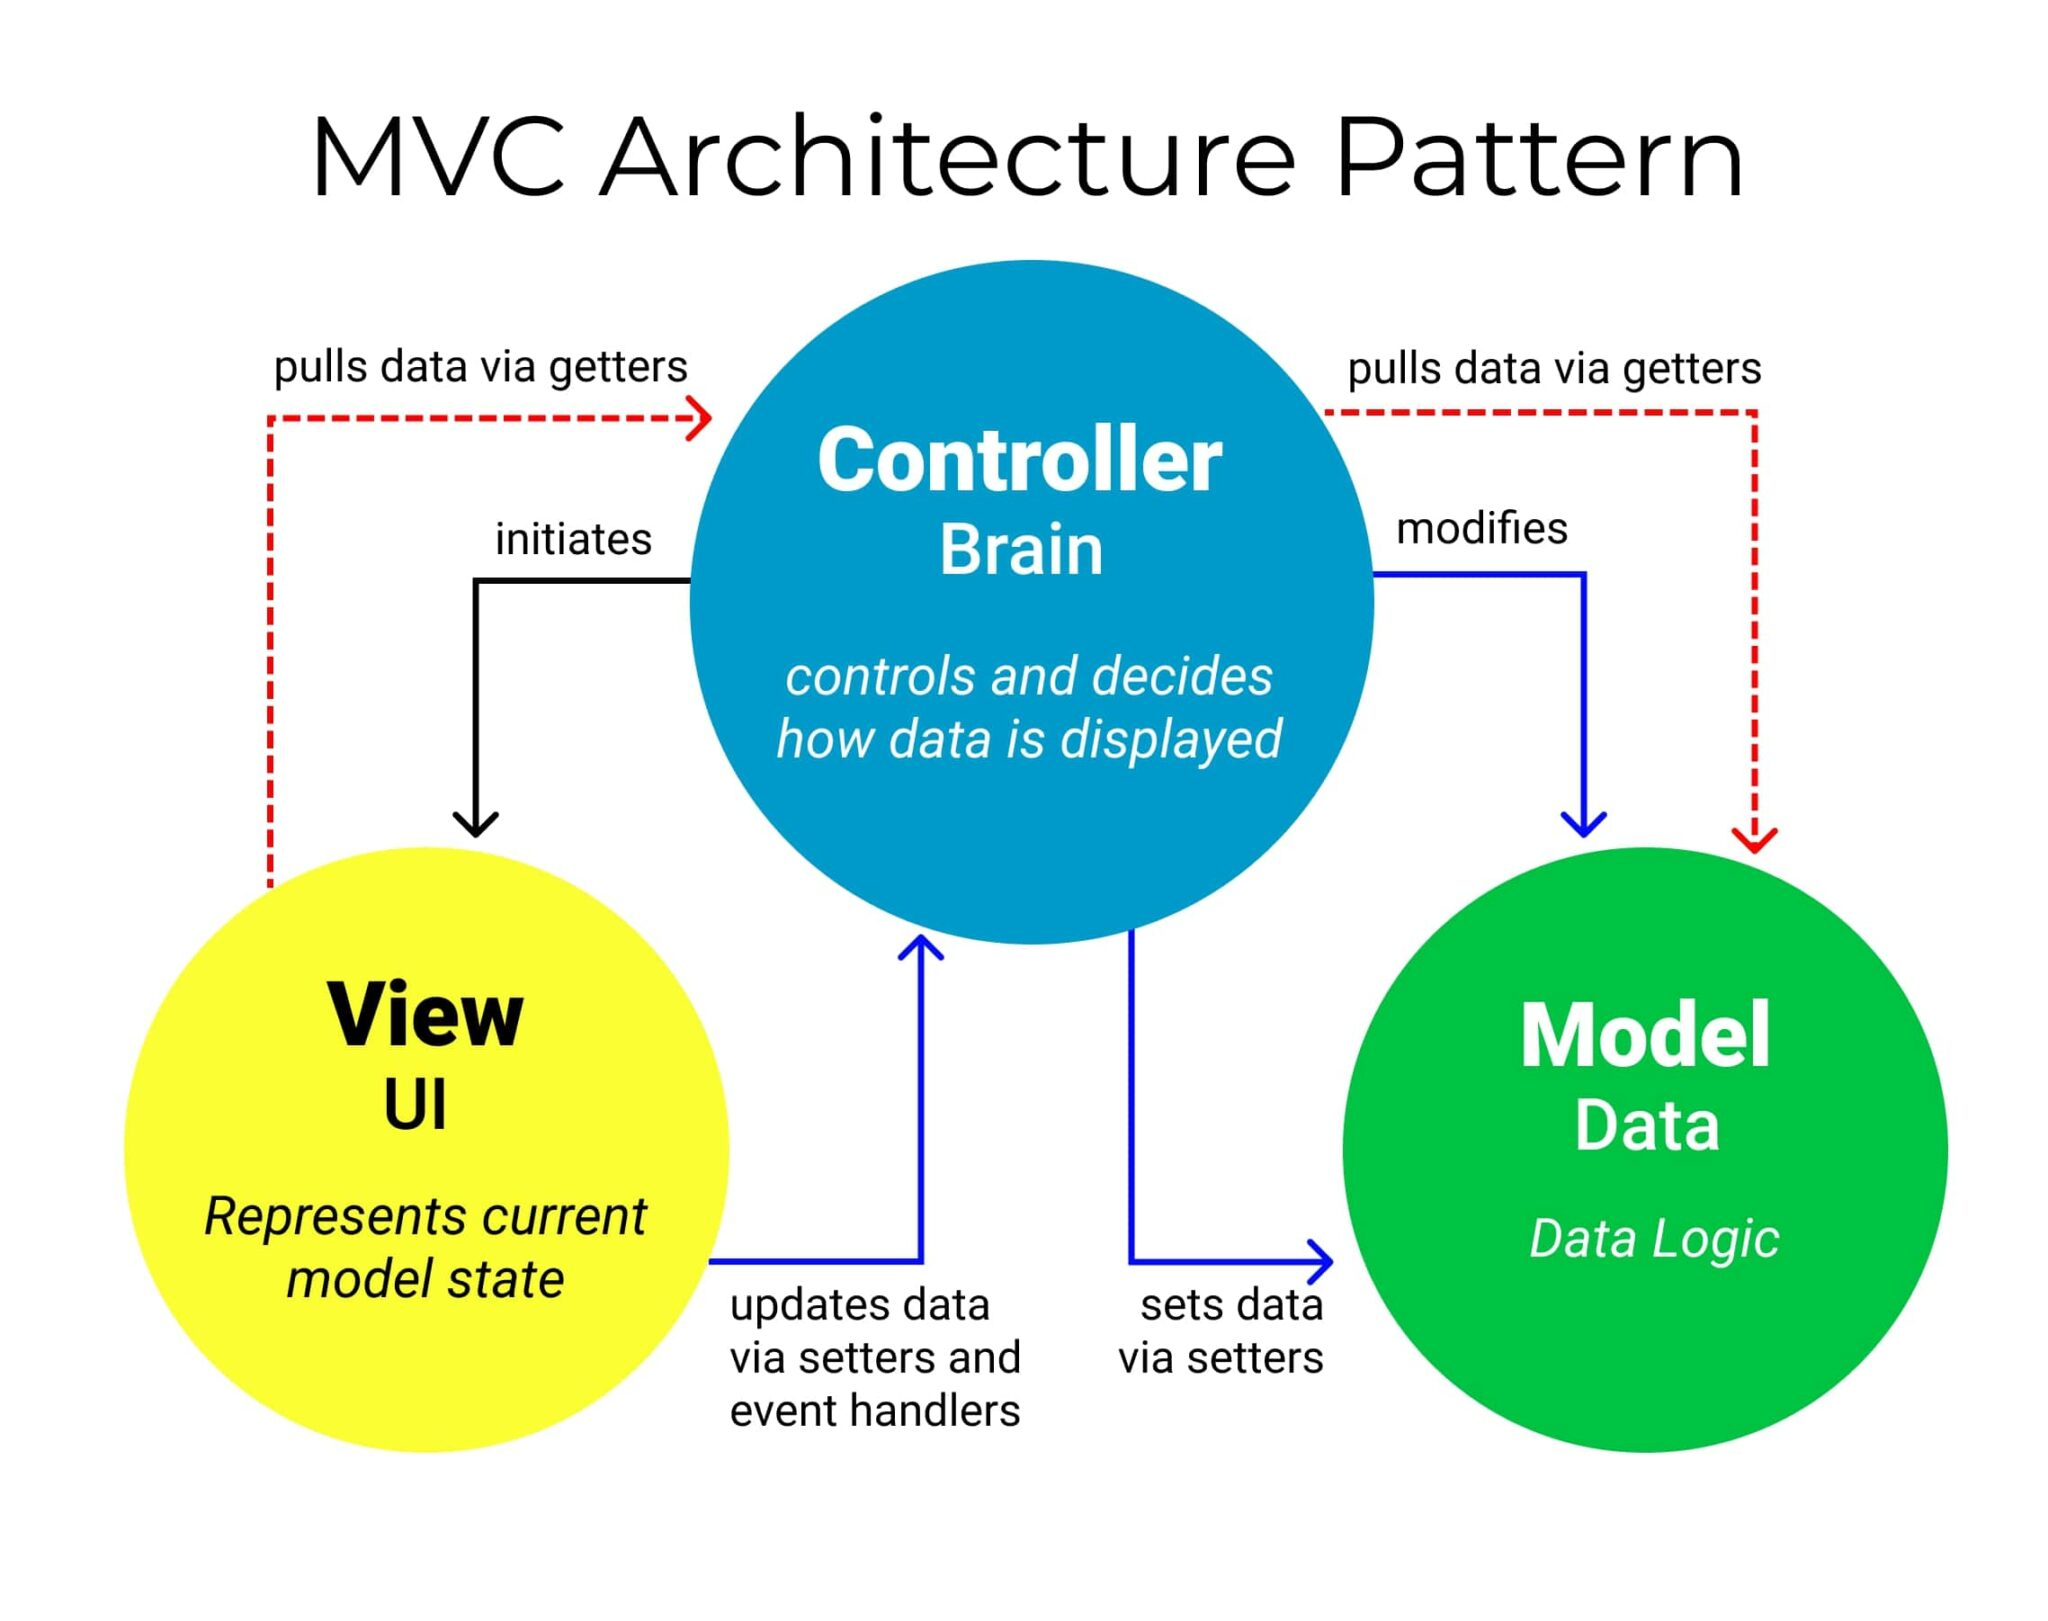
\includegraphics[width=0.8\textwidth]{pictures/MVC.png}
                \caption{Mô hình MVC}
                \label{fig:mvc}
            \end{figure}
        \subsection{Kiến trúc Layered}
            \hspace*{0.6cm}Kiến trúc Layered là một kiểu kiến trúc phần mềm trong đó ứng dụng được chia thành nhiều lớp. Mỗi lớp có nhiệm vụ riêng và tương tác với các lớp khác thông qua các giao diện. Kiến trúc Layered giúp tách biệt các phần của ứng dụng, dễ dàng bảo trì và mở rộng. Ở đây chúng ta có:
            \begin{itemize}
                \item Presentation Layer: Front-end.
                \item Application Layer: mainServer
                \item Data Layer: dbServer và MongoDB.
            \end{itemize}
            \begin{figure}[H]
                \centering
                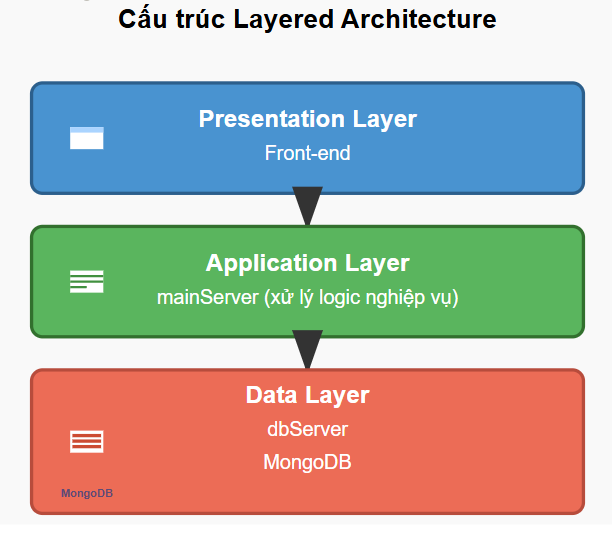
\includegraphics[width=0.8\textwidth]{pictures/Layered.png}
                \caption{Kiến trúc Layered}
                \label{fig:layered}
            \end{figure}
    \section{Cấu trúc thư mục}
        \hspace*{0.6cm}Cấu trúc thư mục của dự án được tổ chức như sau:
        \begin{itemize}
            \item mainServer: Thư mục chứa mã nguồn của Main Server.
            \begin{itemize} 
                \item controllers: Thư mục chứa các controller.
                \item middlewares: Thư mục chứa các middleware.
                \item routes: routes: Thư mục chứa các route.
                \item upload: Thư mục chứa các tệp tải lên.
                \item server.js: Tệp chính của Main Server.
            \end{itemize}
            \item dbServer: Thư mục chứa mã nguồn của Database Server.
            \begin{itemize}
                \item config: Thư mục chứa các tệp cấu hình.
                \item models: Thư mục chứa các mô hình dữ liệu.
                \item seeds: Thư mục chứa các tệp khởi tạo dữ liệu.
                \item dbserver.js: Tệp chính của Database Server.
            \end{itemize}
            \item .env: Tệp cấu hình môi trường.
        \end{itemize}
    \section{Cài đặt}
        \hspace*{0.6cm}Các bước khởi tạo server:
        \begin{itemize}
            \item Khởi tạo NodeJS: \texttt{npm init -y}
            \item Cài đặt dependencies:
            \begin{itemize}
                \item Express: \texttt{npm install express}
                \item Mongoose: \texttt{npm install mongoose}
                \item Multer: \texttt{npm install multer}
                \item Dotenv: \texttt{npm install dotenv}
                \item Cors: \texttt{npm install cors}
                \item Bcrypt: \texttt{npm install bcrypt}
                \item Jsonwebtoken: \texttt{npm install jsonwebtoken}
            \end{itemize}
            \item Tạo server chính: \texttt{touch server.js} và \texttt{touch dbserver.js}
            \item Chạy server bằng lệnh: \texttt{npm start} 
        \end{itemize}
        \hspace*{0.6cm}Các thư viện khác cài đặt trong quá trình phát triển.
    \chapter{MAIN SERVER}
    \section{CONTROLLERS}
        \hspace*{0.6cm}Là nơi chứa logic xử lý cho các endpoint API, thuộc tầng Controller (MVC) hoặc Application Layer (Layered Architecture). Có chức năng:
        \begin{itemize}
            \item Xử lý logic nghiệp vụ: Các hàm trong controller (như loginUser, getDevices) xử lý yêu cầu từ Front-end, gọi API của dbServer để lấy dữ liệu, và trả kết quả.
            \item Điều phối giữa Route và Model: Kết nối các route (trong routes/) với dữ liệu từ dbServer.
        \end{itemize}
        \subsection{deviceController}
            \hspace*{0.6cm}Chứa các hàm xử lý liên quan đến thiết bị, như thêm, sửa, xóa thiết bị. Các hàm này sẽ gọi API của dbServer để thực hiện các thao tác trên cơ sở dữ liệu.
            \subsubsection{Import}
                \hspace*{0.6cm}Thư viện được nhập:
                \begin{lstlisting}
    import axios from "axios";
                \end{lstlisting}
                \begin{itemize}
                    \item \texttt{axios}: Thư viện để gửi yêu cầu HTTP tới server cơ sở dữ liệu.
                \end{itemize}

            \subsubsection{Biến URL}
                \hspace*{0.6cm}Định nghĩa URL server cơ sở dữ liệu:
                \begin{lstlisting}
                const DB_SERVER_URL = process.env.DB_SERVER_URL || "http://localhost:5001";
                \end{lstlisting}
                \begin{itemize}
                    \item \texttt{DB\_SERVER\_URL}: Lấy từ biến môi trường hoặc mặc định \texttt{http://localhost:5001}.
                \end{itemize}

            \subsubsection{Hàm getDevices}
                \hspace*{0.6cm}Hàm xử lý yêu cầu lấy danh sách thiết bị:
                \begin{lstlisting}
    export const getDevices = async (req, res) => {
        try {
            const response = await axios.get(`${DB_SERVER_URL}/db/devices`);
            res.json(response.data);
        } catch (error) {
            res.status(500).json({ message: "Error fetching device list" });
        }
    };
                \end{lstlisting}
                \begin{itemize}
                    \item \texttt{req}, \texttt{res}: Tham số yêu cầu và phản hồi từ framework như Express.js.
                    \item Gửi yêu cầu GET tới \texttt{/db/devices} trên \texttt{DB\_SERVER\_URL}.
                    \item Nếu thành công:
                    \begin{itemize}
                        \item Trả về dữ liệu JSON từ phản hồi của server (\texttt{response.data}).
                    \end{itemize}
                    \item Nếu thất bại:
                    \begin{itemize}
                        \item Trả về mã trạng thái 500 và thông báo lỗi \texttt{\{ message: "Error fetching device list" \}}.
                    \end{itemize}
                \end{itemize}

            \subsubsection{Export}
                \hspace*{0.6cm}Hàm được xuất:
                \begin{lstlisting}
    export default getDevices;
                \end{lstlisting}
                \begin{itemize}
                    \item Xuất hàm để sử dụng trong các tuyến API của ứng dụng Node.js.
                \end{itemize}

            \subsubsection{Chức Năng Chính}
                \begin{itemize}
                    \item \textbf{Lấy Danh Sách Thiết Bị}: Sử dụng \texttt{axios} để gửi yêu cầu GET tới endpoint \texttt{/db/devices} trên server cơ sở dữ liệu.
                    \item \textbf{Xử Lý Phản Hồi}: Trả về danh sách thiết bị dưới dạng JSON nếu thành công, hoặc thông báo lỗi nếu thất bại.
                    \item \textbf{Xử Lý Lỗi}: Trả về mã trạng thái 500 và thông báo lỗi khi không thể lấy dữ liệu.
                    \item \textbf{Tích Hợp API}: Được thiết kế để sử dụng trong các tuyến API, tương thích với Express.js.
                \end{itemize}
        \subsubsection{userController}
            \hspace*{0.6cm}Các hàm API \texttt{registerUser}, \texttt{loginUser}, \texttt{logoutUser}, \texttt{updateAvatar}, \texttt{changePassword}, cùng các hàm hỗ trợ, là các hàm xử lý yêu cầu liên quan đến quản lý người dùng trong ứng dụng Node.js. Sử dụng \texttt{axios} để giao tiếp với server cơ sở dữ liệu, \texttt{jwt} để tạo token xác thực, và \texttt{fs} để quản lý tệp avatar, các hàm này cung cấp các chức năng đăng ký, đăng nhập, đăng xuất, cập nhật avatar và đổi mật khẩu. Báo cáo này phân tích chi tiết mã nguồn, chức năng và thiết kế của các hàm. 
            \subsection{Import}
                \hspace*{0.6cm}Các thư viện được nhập:
                \begin{lstlisting}
    import axios from "axios";
    import jwt from "jsonwebtoken";
    import fs from "fs";
    import path from "path";
    import { fileURLToPath } from "url";
                \end{lstlisting}
                \begin{itemize}
                    \item \texttt{axios}: Gửi yêu cầu HTTP tới server cơ sở dữ liệu.
                    \item \texttt{jwt}: Tạo và xác minh JSON Web Token cho xác thực.
                    \item \texttt{fs}: Quản lý hệ thống tệp (tệp avatar).
                    \item \texttt{path}: Xử lý đường dẫn tệp.
                    \item \texttt{fileURLToPath}: Chuyển URL mô-đun ES thành đường dẫn tệp.
                \end{itemize}

            \subsubsection{Biến và Hằng}
                \hspace*{0.6cm}Định nghĩa URL và đường dẫn:
                \begin{lstlisting}
    const DB_SERVER_URL = process.env.DB_SERVER_URL || "http://localhost:5001";

    const __filename = fileURLToPath(import.meta.url);
    const __dirname = path.dirname(__filename);
                \end{lstlisting}
                \begin{itemize}
                    \item \texttt{DB\_SERVER\_URL}: URL server cơ sở dữ liệu, mặc định \texttt{http://localhost:5001}.
                    \item \texttt{\_\_filename}, \texttt{\_\_dirname}: Đường dẫn tệp hiện tại, hỗ trợ mô-đun ES.
                \end{itemize}

            \subsubsection{Hàm Kiểm Tra Đầu Vào}
                \hspace*{0.6cm}Các hàm kiểm tra dữ liệu đầu vào:
                \begin{lstlisting}
    const isValidEmail = (email) => {
        const emailRegex = /^[^\s@]+@[^\s@]+\.[^\s@]+$/;
        return emailRegex.test(email);
    };

    const validateRegisterInput = (username, email, password) => {
        if (!username || username.length < 3) {
            return "Username must be at least 3 characters";
        }
        if (!email || !isValidEmail(email)) {
            return "Invalid email";
        }
        if (!password || password.length < 6) {
            return "Password must be at least 6 characters";
        }
        return null;
    };

    const validateLoginInput = (email, password) => {
        if (!email || !isValidEmail(email)) {
            return "Invalid email";
        }
        if (!password || password.length < 6) {
            return "Password must be at least 6 characters";
        }
        return null;
    };

    const validateChangePasswordInput = (oldPassword, newPassword) => {
        if (!oldPassword || oldPassword.length < 6) {
            return "Password must be at least 6 characters";
        }
        if (!newPassword || newPassword.length < 6) {
            return "Password must be at least 6 characters";
        }
        if (oldPassword === newPassword) {
            return "New password must differ from old password";
        }
        return null;
    };
                \end{lstlisting}
                \begin{itemize}
                    \item \texttt{isValidEmail}: Kiểm tra định dạng email bằng regex.
                    \item \texttt{validateRegisterInput}: Kiểm tra \texttt{username} (ít nhất 3 ký tự, sử dụng $\geq 3$), \texttt{email} (hợp lệ), \texttt{password} (ít nhất 6 ký tự, sử dụng $\geq 6$).
                    \item \texttt{validateLoginInput}: Kiểm tra \texttt{email} (hợp lệ), \texttt{password} (ít nhất 6 ký tự, sử dụng $\geq 6$).
                    \item \texttt{validateChangePasswordInput}: Kiểm tra \texttt{oldPassword}, \texttt{newPassword} (ít nhất 6 ký tự, sử dụng $\geq 6$, và khác nhau).
                \end{itemize}

            \subsubsection{Hàm registerUser}
                \hspace*{0.6cm}Hàm đăng ký người dùng:
                \begin{lstlisting}
export const registerUser = async (req, res) => {
    const { username, email, password } = req.body;
    try {
        const validationError = validateRegisterInput(username, email, password);
        if (validationError) {
            return res.status(400).json({ message: validationError });
        }

        const response = await axios.get(`${DB_SERVER_URL}/db/users/email/${email}`);
        if (response.status === 200) {
            return res.status(400).json({ message: "Email already exists" });
        }

        const newUser = await axios.post(`${DB_SERVER_URL}/db/users`, { username, email, password });
        res.status(201).json({ message: "Registration successful" });
    } catch (err) {
        if (err.response && err.response.status === 404) {
            try {
                await axios.post(`${DB_SERVER_URL}/db/users`, { username, email, password });
                res.status(201).json({ message: "Registration successful" });
            } catch (createErr) {
                res.status(500).json({ message: "Error registering user" });
            }
        } else {
            res.status(500).json({ message: "Error registering user" });
        }
    }
};
            \end{lstlisting}
                \begin{itemize}
                    \item Kiểm tra đầu vào với \texttt{validateRegisterInput}.
                    \item Kiểm tra email tồn tại bằng GET \texttt{/db/users/email/:email}.
                    \item Nếu email đã tồn tại, trả về lỗi 400.
                    \item Nếu email không tồn tại (404), tạo người dùng mới bằng POST \texttt{/db/users}.
                    \item Trả về thông báo thành công (201) hoặc lỗi (500).
                \end{itemize}

            \subsubsection{Hàm loginUser}
                \hspace*{0.6cm}Hàm đăng nhập người dùng:
                \begin{lstlisting}
export const loginUser = async (req, res) => {
    const { email, password } = req.body;
    try {
        const validationError = validateLoginInput(email, password);
        if (validationError) {
            console.log("Validation error:", validationError);
            return res.status(400).json({ message: validationError });
        }

        console.log("Logging in:", email);
        const response = await axios.get(`${DB_SERVER_URL}/db/users/email/${email}`);
        const user = response.data;

        console.log("User found:", user.email);
        const isMatch = await bcryptCompare(password, user.password);
        if (!isMatch) {
            console.log("Incorrect password for:", email);
            return res.status(401).json({ message: "Invalid login credentials" });
        }

        console.log("Login successful, generating token...");
        const token = jwt.sign({ id: user._id }, process.env.JWT_SECRET, { expiresIn: "1d" });
        res.cookie("authToken", token, {
            httpOnly: true,
            secure: process.env.NODE_ENV === "production",
            sameSite: "lax",
            maxAge: 24 * 60 * 60 * 1000,
        });
        res.json({ username: user.username, avatar: user.avatar });
    } catch (err) {
        if (err.response && err.response.status === 404) {
            console.log("User not found:", email);
            return res.status(401).json({ message: "Invalid login credentials" });
        }
        console.error("Login error:", err.message);
        res.status(500).json({ message: "Login error" });
    }
};
                \end{lstlisting}
                \begin{itemize}
                    \item Kiểm tra đầu vào với \texttt{validateLoginInput}.
                    \item Tìm người dùng bằng GET \texttt{/db/users/email/:email}.
                    \item So sánh mật khẩu với \texttt{bcryptCompare} (yêu cầu \texttt{bcryptjs}).
                    \item Nếu mật khẩu khớp, tạo JWT và lưu vào cookie \texttt{authToken}.
                    \item Trả về \texttt{username} và \texttt{avatar}, hoặc lỗi nếu thất bại.
                \end{itemize}

            \subsubsection{Hàm logoutUser}
                \hspace*{0.6cm}Hàm đăng xuất người dùng:
                \begin{lstlisting}
                export const logoutUser = async (req, res) => {
                    res.clearCookie("authToken");
                    res.json({ message: "Logout successful" });
                };
                \end{lstlisting}
                \begin{itemize}
                    \item Xóa cookie \texttt{authToken}.
                    \item Trả về thông báo thành công.
                \end{itemize}

            \subsubsection{Hàm updateAvatar}
                \hspace*{0.6cm}Hàm cập nhật avatar:
                \begin{lstlisting}
export const updateAvatar = async (req, res) => {
    try {
        const userId = req.user.id;
        console.log("User ID:", userId);
        const response = await axios.get(`${DB_SERVER_URL}/db/users/${userId}`);
        const user = response.data;

        if (!req.file) {
            console.log("No file uploaded");
            return res.status(400).json({ message: "No file uploaded" });
        }

        console.log("File uploaded:", req.file);

        const uploadDir = path.join(__dirname, "../upload/avatars");
        if (!uploadDir) {
            console.log("Creating upload/avatars directory");
            fs.mkdirSync(uploadDir, { recursive: true });
        }

        if (user.avatar) {
            const oldAvatarFilename = path.basename(user.avatar);
            const oldAvatarPath = path.join(uploadDir, oldAvatarFilename);
            try {
                if (fs.existsSync(oldAvatarPath)) {
                    console.log(`Deleting old avatar file: ${oldAvatarPath}`);
                    fs.unlinkSync(oldAvatarPath);
                } else {
                    console.log(`Old avatar file not found: ${oldAvatarPath}`);
                }
            } catch (err) {
                console.error("Error deleting old avatar file:", err.message);
            }
        }

        const avatarPath = `/avatars/${req.file.filename}`;
        await axios.put(`${DB_SERVER_URL}/db/users/${userId}`, { avatar: avatarPath });
        console.log("Updated avatar in database:", avatarPath);

        res.json({ avatar: avatarPath });
    } catch (err) {
        console.error("Error updating avatar:", err.message);
        if (req.file) {
            const newAvatarPath = path.join(__dirname, "../upload/avatars", req.file.filename);
            try {
                if (fs.existsSync(newAvatarPath)) {
                    console.log(`Deleting new file due to error: ${newAvatarPath}`);
                    fs.unlinkSync(newAvatarPath);
                }
            } catch (err) {
                console.error("Error deleting new file:", err.message);
            }
        }
        res.status(500).json({ message: err.message || "Error updating avatar" });
    }
};
                \end{lstlisting}
                \begin{itemize}
                    \item Lấy \texttt{userId} từ \texttt{req.user.id} (giả định middleware xác thực).
                    \item Kiểm tra và tạo thư mục \texttt{upload/avatars} nếu chưa tồn tại.
                    \item Xóa avatar cũ nếu có.
                    \item Lưu đường dẫn avatar mới và cập nhật trong cơ sở dữ liệu bằng PUT \texttt{/db/users/:id}.
                    \item Nếu lỗi, xóa tệp mới tải lên và trả về thông báo lỗi.
                \end{itemize}

            \subsubsection{Hàm changePassword}
                \hspace*{0.6cm}Hàm đổi mật khẩu:
                \begin{lstlisting}
export const changePassword = async (req, res) => {
    const { oldPassword, newPassword } = req.body;
    try {
        const validationError = validateChangePasswordInput(oldPassword, newPassword);
        if (validationError) {
            return res.status(400).json({ message: validationError });
        }

        const userId = req.user.id;
        const response = await axios.get(`${DB_SERVER_URL}/db/users/${userId}`);
        const user = response.data;

        const isMatch = await bcryptCompare(oldPassword, user.password);
        if (!isMatch) {
            return res.status(401).json({ message: "Incorrect old password" });
        }

        await axios.put(`${DB_SERVER_URL}/db/users/${userId}`, { password: newPassword });

        res.json({ message: "Password change successful" });
    } catch (err) {
        console.error("Error changing password:", err.message);
        res.status(500).json({ message: "Error changing password" });
    }
};
                \end{lstlisting}
                \begin{itemize}
                    \item Kiểm tra đầu vào với \texttt{validateChangePasswordInput}.
                    \item So sánh \texttt{oldPassword} với mật khẩu hiện tại bằng \texttt{bcryptCompare}.
                    \item Cập nhật mật khẩu mới bằng PUT \texttt{/db/users/:id}.
                    \item Trả về thông báo thành công hoặc lỗi.
                \end{itemize}

            \subsubsection{Hàm bcryptCompare}
                \hspace*{0.6cm}Hàm so sánh mật khẩu:
                \begin{lstlisting}
    const bcryptCompare = async (plainPassword, hashedPassword) => {
        const bcrypt = await import("bcryptjs");
        return await bcrypt.compare(plainPassword, hashedPassword);
    };
                \end{lstlisting}
                \begin{itemize}
                    \item Tạm thời nhập \texttt{bcryptjs} và so sánh mật khẩu, yêu cầu cài đặt \texttt{bcryptjs} trên server chính.
                \end{itemize}

            \subsubsection{Chức Năng Chính}
                \begin{itemize}
                    \item \textbf{Đăng Ký Người Dùng}: Kiểm tra đầu vào, kiểm tra email tồn tại, tạo người dùng mới.
                    \item \textbf{Đăng Nhập Người Dùng}: Kiểm tra thông tin đăng nhập, tạo JWT, lưu cookie xác thực.
                    \item \textbf{Đăng Xuất Người Dùng}: Xóa cookie xác thực.
                    \item \textbf{Cập Nhật Avatar}: Xóa avatar cũ, lưu avatar mới, cập nhật cơ sở dữ liệu.
                    \item \textbf{Đổi Mật Khẩu}: Kiểm tra mật khẩu cũ, cập nhật mật khẩu mới.
                    \item \textbf{Kiểm Tra Đầu Vào}: Đảm bảo dữ liệu hợp lệ cho đăng ký, đăng nhập, đổi mật khẩu.
                \end{itemize}
    \section{ROUTES}
        \hspace*{0.6cm}Là nơi định tuyến yêu cầu từ Front-end đến controller, thuộc tầng Controller (MVC) hoặc Application Layer (Layered Architecture). Có chức năng:
        \begin{itemize}
            \item Định nghĩa endpoint API: Xác định các URL (như /api/users/login, /api/devices) và phương thức HTTP (GET, POST, v.v.).
            \item Điều phối yêu cầu: Chuyển yêu cầu từ Front-end đến các hàm xử lý trong controllers/ (như loginUser, getDevices).
            \item Áp dụng middleware: Thêm các middleware (như authenticateToken, upload) trước khi gọi controller.
        \end{itemize}
        \subsection{deviceRoute}
            \hspace*{0.6cm}Xác định endpoint như GET /api/devices để lấy danh sách thiết bị, gọi hàm getDevices trong deviceController.js và sử dụng authenticateToken để kiểm tra token trước khi xử lý
            \subsubsection{Import}
                \hspace*{0.6cm}Các thư viện và thành phần được nhập:
                \begin{lstlisting}
    import express from "express";
    import { getDevices } from "../controllers/deviceController.js";
    import { authenticateToken } from "../middleware/auth.js";
                \end{lstlisting}
                \begin{itemize}
                    \item \texttt{express}: Framework để tạo router và xử lý yêu cầu HTTP.
                    \item \texttt{getDevices}: Hàm xử lý từ \texttt{deviceController} để lấy danh sách thiết bị.
                    \item \texttt{authenticateToken}: Middleware xác thực token từ \texttt{auth}.
                \end{itemize}

            \subsubsection{Định Nghĩa Router}
                \hspace*{0.6cm}Tạo một router Express:
                \begin{lstlisting}
                const router = express.Router();
                \end{lstlisting}
                \begin{itemize}
                    \item \texttt{router}: Một instance của \texttt{express.Router} để định nghĩa các tuyến API.
                \end{itemize}

            \subsubsection{Tuyến API}
                \hspace*{0.6cm}Định nghĩa tuyến GET:
                \begin{lstlisting}
    router.get("/", authenticateToken, getDevices);
                \end{lstlisting}
                \begin{itemize}
                    \item \texttt{router.get("/")}: Định nghĩa tuyến GET cho đường dẫn gốc (\texttt{/}).
                    \item \texttt{authenticateToken}: Middleware kiểm tra token xác thực trước khi xử lý yêu cầu.
                    \item \texttt{getDevices}: Hàm xử lý trả về danh sách thiết bị.
                \end{itemize}
            \subsubsection{Export}
                \hspace*{0.6cm}Xuất router để sử dụng trong ứng dụng:
                \begin{lstlisting}
    export default router;
                \end{lstlisting}
                \begin{itemize}
                    \item Xuất \texttt{router} để tích hợp vào ứng dụng Express chính.
                \end{itemize}

            \subsubsection{Chức Năng Chính}
                \hspace*{0.6cm}Tệp định tuyến cung cấp một tuyến API để lấy danh sách thiết bị:
                \begin{itemize}
                    \item \textbf{Định Tuyến Yêu Cầu}: Xử lý yêu cầu GET tại \texttt{/} để trả về danh sách thiết bị.
                    \item \textbf{Xác Thực Yêu Cầu}: Sử dụng middleware \texttt{authenticateToken} để đảm bảo chỉ người dùng đã đăng nhập mới truy cập được.
                    \item \textbf{Tích Hợp Hàm Xử Lý}: Gọi \texttt{getDevices} để lấy dữ liệu từ server cơ sở dữ liệu.
                    \item \textbf{Thiết Kế Mô-đun}: Sử dụng \texttt{express.Router} để tổ chức tuyến API một cách độc lập, dễ bảo trì.
                \end{itemize}
        \subsection{userRoute}
            \hspace*{0.6cm}Tệp định nghĩa route cho người dùng: Xác định các endpoint như POST /api/users/login, POST /api/users/register, POST /api/users/change-password...Gọi các hàm như loginUser, registerUser, changePassword trong usersController.js và sử dụng authenticateToken (xác thực token) hoặc upload (xử lý file upload) cho một số route.
            \subsubsection{Import}
                \hspace*{0.6cm}Các thư viện và thành phần được nhập:
                \begin{lstlisting}
    import express from "express";
    import { registerUser, loginUser, logoutUser, updateAvatar, changePassword } from "../controllers/usersController.js";
    import { authenticateToken } from "../middleware/auth.js";
    import upload from "../middleware/upload.js";
                \end{lstlisting}
                \begin{itemize}
                    \item \texttt{express}: Framework để tạo router và xử lý yêu cầu HTTP.
                    \item \texttt{registerUser}, \texttt{loginUser}, \texttt{logoutUser}, \texttt{updateAvatar}, \texttt{changePassword}: Các hàm xử lý từ \texttt{usersController}.
                    \item \texttt{authenticateToken}: Middleware xác thực token từ \texttt{auth}.
                    \item \texttt{upload}: Middleware xử lý tải tệp từ \texttt{upload}.
                \end{itemize}

            \subsubsection{Định Nghĩa Router}
                \hspace*{0.6cm}Tạo một router Express:
                \begin{lstlisting}
    const router = express.Router();
                \end{lstlisting}
                \begin{itemize}
                    \item \texttt{router}: Một instance của \texttt{express.Router} để định nghĩa các tuyến API.
                \end{itemize}

            \subsubsection{Tuyến API}
                \hspace*{0.6cm}Định nghĩa các tuyến API cho quản lý người dùng:
                \begin{lstlisting}
    router.post("/register", registerUser);
    router.post("/login", loginUser);
    router.post("/logout", logoutUser);
    router.post("/update-avatar", authenticateToken, upload.single("avatar"), updateAvatar);
    router.post("/change-password", authenticateToken, changePassword);

    router.get('/verify-token', authenticateToken, (req, res) => {
        res.json({ valid: true });
    });
                \end{lstlisting}
                \begin{itemize}
                    \item \texttt{router.post("/register", registerUser)}: Tuyến POST để đăng ký người dùng mới.
                    \item \texttt{router.post("/login", loginUser)}: Tuyến POST để đăng nhập người dùng.
                    \item \texttt{router.post("/logout", logoutUser)}: Tuyến POST để đăng xuất người dùng.
                    \item \texttt{router.post("/update-avatar", authenticateToken, upload.single("avatar"), updateAvatar)}: Tuyến POST để cập nhật avatar, yêu cầu xác thực và tải tệp.
                    \item \texttt{router.post("/change-password", authenticateToken, changePassword)}: Tuyến POST để đổi mật khẩu, yêu cầu xác thực.
                    \item \texttt{router.get("/verify-token", authenticateToken, ...)}: Tuyến GET để xác minh token, trả về \texttt{\{ valid: true \}} nếu token hợp lệ.
                \end{itemize}

            \subsubsection{Export}
                \hspace*{0.6cm}Xuất router để sử dụng trong ứng dụng:
                \begin{lstlisting}
    export default router;
                \end{lstlisting}
                \begin{itemize}
                    \item Xuất \texttt{router} để tích hợp vào ứng dụng Express chính.
                \end{itemize}

            \subsubsection{Chức Năng Chính}
                \hspace*{0.6cm}Tệp định tuyến cung cấp các tuyến API để quản lý người dùng:
                \begin{itemize}
                    \item \textbf{Định Tuyến Yêu Cầu Người Dùng}: Xử lý các yêu cầu POST cho đăng ký, đăng nhập, đăng xuất, cập nhật avatar, và đổi mật khẩu; yêu cầu GET để xác minh token.
                    \item \textbf{Bảo Mật Yêu Cầu}: Sử dụng middleware \texttt{authenticateToken} để bảo vệ các tuyến \texttt{update-avatar}, \texttt{change-password}, và \texttt{verify-token}.
                    \item \textbf{Xử Lý Tệp Tải Lên}: Sử dụng middleware \texttt{upload.single("avatar")} để xử lý tệp avatar trong tuyến \texttt{update-avatar}.
                    \item \textbf{Tích Hợp Hàm Xử Lý}: Gọi các hàm từ \texttt{usersController} để thực hiện logic quản lý người dùng.
                    \item \textbf{Thiết Kế Mô-đun}: Sử dụng \texttt{express.Router} để tổ chức các tuyến API một cách độc lập, dễ bảo trì.
                \end{itemize}
    \section{MIDDLEWARE}
        \hspace*{0.6cm}Là nơi chứa các middleware dùng để:
        \begin{itemize}
            \item Xử lý trung gian: Thực hiện các tác vụ trước khi yêu cầu đến controller (như xác thực, xử lý file upload).
            \item Kiểm soát luồng yêu cầu: Kiểm tra, biến đổi hoặc chặn yêu cầu dựa trên điều kiện.
        \end{itemize}
        \subsection{auth}
            \hspace*{0.6cm}Middleware xác thực token người dùng, kiểm tra tính hợp lệ của token trong cookie và giải mã thông tin người dùng.
            \subsubsection{Import}
                \hspace*{0.6cm}Thư viện được nhập:
                \begin{lstlisting}
    import jwt from "jsonwebtoken";
                \end{lstlisting}
                \begin{itemize}
                    \item \texttt{jwt}: Thư viện để xác minh và giải mã JSON Web Token.
                \end{itemize}

            \subsubsection{Hàm authenticateToken}
                \hspace*{0.6cm}Middleware xác minh token:
                \begin{lstlisting}
    export const authenticateToken = (req, res, next) => {
        const token = req.cookies.authToken;
        if (!token) {
            return res.status(401).json({ message: "Not logged in" });
        }

        jwt.verify(token, process.env.JWT_SECRET, (err, user) => {
            if (err) {
                return res.status(403).json({ message: "Invalid token" });
            }
            req.user = user;
            next();
        });
    };
                \end{lstlisting}
                \begin{itemize}
                    \item \texttt{req}, \texttt{res}, \texttt{next}: Tham số chuẩn của middleware Express.
                    \item Lấy \texttt{token} từ cookie \texttt{authToken}.
                    \item Nếu không có token, trả về lỗi 401 với thông báo \texttt{"Not logged in"}.
                    \item Sử dụng \texttt{jwt.verify} để xác minh token với \texttt{JWT\_SECRET}.
                    \item Nếu token không hợp lệ, trả về lỗi 403 với thông báo \texttt{"Invalid token"}.
                    \item Nếu hợp lệ, gán thông tin người dùng vào \texttt{req.user} và gọi \texttt{next()} để chuyển tiếp yêu cầu.
                \end{itemize}

            \subsubsection{Export}
                \hspace*{0.6cm}Xuất middleware để sử dụng trong các tuyến API:
                \begin{lstlisting}
    export default authenticateToken;
                \end{lstlisting}
                \begin{itemize}
                    \item Xuất \texttt{authenticateToken} để tích hợp vào các tuyến API của ứng dụng Express.
                \end{itemize}

            \subsubsection{Chức Năng Chính}
                \hspace*{0.6cm}Middleware \texttt{authenticateToken} cung cấp xác thực cho các yêu cầu API:
                \begin{itemize}
                    \item \textbf{Xác Minh Token}: Kiểm tra sự tồn tại và tính hợp lệ của JWT trong cookie \texttt{authToken}.
                    \item \textbf{Bảo Vệ Tuyến API}: Từ chối các yêu cầu không có token (401) hoặc token không hợp lệ (403).
                    \item \textbf{Gán Thông Tin Người Dùng}: Thêm thông tin người dùng vào \texttt{req.user} nếu token hợp lệ.
                    \item \textbf{Tích Hợp Express}: Sử dụng cơ chế middleware để dễ dàng áp dụng cho các tuyến API cần xác thực.
                \end{itemize}
        \subsection{upload}
            \hspace*{0.6cm}Middleware xử lý tải tệp, sử dụng thư viện \texttt{multer} để quản lý việc tải lên tệp avatar của người dùng.
            \subsubsection{Import}
                \hspace*{0.6cm}Các thư viện được nhập:
                \begin{lstlisting}
    import multer from "multer";
    import path from "path";
    import { fileURLToPath } from "url";
    import fs from "fs";
                \end{lstlisting}
                \begin{itemize}
                    \item \texttt{multer}: Thư viện để xử lý tải lên tệp trong Express.
                    \item \texttt{path}: Xử lý đường dẫn tệp.
                    \item \texttt{fileURLToPath}: Chuyển URL mô-đun ES thành đường dẫn tệp.
                    \item \texttt{fs}: Quản lý hệ thống tệp (tạo thư mục, kiểm tra tệp).
                \end{itemize}

            \subsubsection{Biến Đường Dẫn}
                \hspace*{0.6cm}Định nghĩa đường dẫn tệp hiện tại:
                \begin{lstlisting}
    const __filename = fileURLToPath(import.meta.url);
    const __dirname = path.dirname(__filename);
                \end{lstlisting}
                \begin{itemize}
                    \item \texttt{\_\_filename}, \texttt{\_\_dirname}: Đường dẫn tệp hiện tại, hỗ trợ mô-đun ES.
                \end{itemize}

            \subsubsection{Cấu Hình Lưu Trữ}
                \hspace*{0.6cm}Cấu hình lưu trữ cho \texttt{multer}:
                \begin{lstlisting}
    const storage = multer.diskStorage({
        destination: (req, file, cb) => {
            const uploadDir = path.join(__dirname, "../upload/avatars");
            if (!fs.existsSync(uploadDir)) {
                fs.mkdirSync(uploadDir, { recursive: true });
            }
            cb(null, uploadDir);
        },
        filename: (req, file, cb) => {
            const uniqueSuffix = Date.now() + "-" + Math.round(Math.random() * 1e9);
            cb(null, uniqueSuffix + path.extname(file.originalname));
        },
    });
                \end{lstlisting}
                \begin{itemize}
                    \item \texttt{destination}: Tạo thư mục \texttt{upload/avatars} nếu chưa tồn tại, đặt đích lưu trữ là thư mục này.
                    \item \texttt{filename}: Tạo tên tệp duy nhất bằng thời gian hiện tại và số ngẫu nhiên, giữ nguyên phần mở rộng của tệp gốc.
                \end{itemize}

            \subsubsection{Cấu Hình Multer}
                \hspace*{0.6cm}Tạo middleware \texttt{upload} với \texttt{multer}:
                \begin{lstlisting}
    const upload = multer({
        storage,
        limits: { fileSize: 5 * 1024 * 1024 },
        fileFilter: (req, file, cb) => {
            const filetypes = /jpeg|jpg|png/;
            const extname = filetypes.test(path.extname(file.originalname).
            toLowerCase());
            const mimetype = filetypes.test(file.mimetype);
            if (extname && mimetype) {
                return cb(null, true);
            }
            cb(new Error("Only JPEG or PNG files are accepted"));
        },
    });
                \end{lstlisting}
                \begin{itemize}
                    \item \texttt{storage}: Sử dụng cấu hình lưu trữ đã định nghĩa.
                    \item \texttt{limits}: Giới hạn kích thước tệp tối đa 5MB (\texttt{5 * 1024 * 1024} byte).
                    \item \texttt{fileFilter}: Chỉ chấp nhận tệp JPEG hoặc PNG dựa trên phần mở rộng và loại MIME, trả về lỗi nếu không hợp lệ.
                \end{itemize}

            \subsubsection{Export}
                \hspace*{0.6cm}Xuất middleware để sử dụng trong các tuyến API:
                \begin{lstlisting}
    export default upload;
                \end{lstlisting}
                \begin{itemize}
                    \item Xuất \texttt{upload} để tích hợp vào các tuyến API Express, ví dụ: tuyến \texttt{update-avatar}.
                \end{itemize}

            \subsubsection{Chức Năng Chính}
                \hspace*{0.6cm}Middleware \texttt{upload} cung cấp xử lý tải lên tệp hình ảnh:
                \begin{itemize}
                    \item \textbf{Xử Lý Tệp Tải Lên}: Sử dụng \texttt{multer} để nhận và lưu tệp hình ảnh vào thư mục \texttt{upload/avatars}.
                    \item \textbf{Tạo Tên Tệp Duy Nhất}: Tạo tên tệp dựa trên thời gian và số ngẫu nhiên để tránh xung đột.
                    \item \textbf{Giới Hạn và Lọc Tệp}: Giới hạn kích thước tệp 5MB, chỉ chấp nhận định dạng JPEG hoặc PNG.
                    \item \textbf{Quản Lý Thư Mục}: Tự động tạo thư mục \texttt{upload/avatars} nếu chưa tồn tại.
                    \item \textbf{Tích Hợp Express}: Middleware dễ dàng áp dụng cho các tuyến API cần tải lên tệp.
                \end{itemize}
    \section{SERVER}
        \hspace*{0.6cm}Là Application Layer, xử lý logic và điều phối giữa Front-end và dbServer.
        \subsection{Import}
            \hspace*{0.6cm}Các thư viện và mô-đun được nhập:
            \begin{lstlisting}
    import express from "express";
    import dotenv from "dotenv";
    import deviceRoutes from "./routes/deviceRoutes.js";
    import userRoutes from "./routes/usersRoute.js";
    import { createRequire } from "module";
    import http from "http";
    import cookieParser from "cookie-parser";
    import path from "path";
    import { fileURLToPath } from "url";
            \end{lstlisting}
            \begin{itemize}
                \item \texttt{express}: Framework để tạo server và xử lý yêu cầu HTTP.
                \item \texttt{dotenv}: Tải biến môi trường từ tệp \texttt{.env}.
                \item \texttt{deviceRoutes}, \texttt{userRoutes}: Các tuyến API cho thiết bị và người dùng.
                \item \texttt{createRequire}: Hỗ trợ nhập CommonJS trong mô-đun ES.
                \item \texttt{http}: Tạo server HTTP cho Socket.IO.
                \item \texttt{cookieParser}: Xử lý cookie trong yêu cầu.
                \item \texttt{path}, \texttt{fileURLToPath}: Xử lý đường dẫn tệp.
            \end{itemize}

        \subsection{Biến Đường Dẫn}
            \hspace*{0.6cm}Định nghĩa đường dẫn tệp hiện tại:
            \begin{lstlisting}
    const __filename = fileURLToPath(import.meta.url);
    const __dirname = path.dirname(__filename);
            \end{lstlisting}
            \begin{itemize}
                \item \texttt{\_\_filename}, \texttt{\_\_dirname}: Đường dẫn tệp hiện tại, hỗ trợ mô-đun ES.
            \end{itemize}

        \subsection{Cấu Hình Môi Trường}
            \hspace*{0.6cm}Tải biến môi trường từ tệp \texttt{.env}:
            \begin{lstlisting}
    dotenv.config({ path: path.join(__dirname, "../.env") });
            \end{lstlisting}
            \begin{itemize}
                \item \texttt{dotenv.config}: Tải các biến môi trường từ tệp \texttt{.env} trong thư mục gốc.
            \end{itemize}

        \subsection{Khởi Tạo Server}
            \hspace*{0.6cm}Tạo ứng dụng Express và server HTTP:
            \begin{lstlisting}
    const app = express();
    const server = http.createServer(app);
            \end{lstlisting}
            \begin{itemize}
                \item \texttt{app}: Instance của \texttt{express} để xử lý yêu cầu HTTP.
                \item \texttt{server}: Server HTTP để hỗ trợ Socket.IO.
            \end{itemize}

        \subsection{Cấu Hình Socket.IO}
            \hspace*{0.6cm}Khởi tạo Socket.IO với CORS:
            \begin{lstlisting}
    const require = createRequire(import.meta.url);
    const socketIo = require("socket.io");

    const allowedOrigins = [
        "http://localhost:5173",
        "http://192.168.1.10:5173",
        "http://localhost:3000",
    ];

    const io = socketIo(server, {
        cors: {
            origin: allowedOrigins,
            methods: ["GET", "POST", "OPTIONS"],
            credentials: true,
        },
        pingTimeout: 60000,
        pingInterval: 25000,
    });
            \end{lstlisting}
            \begin{itemize}
                \item Nhập \texttt{socket.io} qua CommonJS vì mô-đun ES không hỗ trợ trực tiếp.
                \item \texttt{allowedOrigins}: Danh sách các nguồn được phép cho CORS.
                \item \texttt{io}: Instance Socket.IO với cấu hình CORS, thời gian chờ 60 giây, và kiểm tra kết nối mỗi 25 giây.
            \end{itemize}

        \subsection{Middleware}
            \hspace*{0.6cm}Cấu hình middleware cho ứng dụng:
            \begin{lstlisting}
    app.use((req, res, next) => {
        const origin = req.headers.origin;
        if (allowedOrigins.includes(origin)) {
            res.setHeader("Access-Control-Allow-Origin", origin);
            res.setHeader("Access-Control-Allow-Credentials", "true");
            res.setHeader("Access-Control-Allow-Methods", "GET, POST, OPTIONS");
            res.setHeader("Access-Control-Allow-Headers", "Content-Type, Authorization");
        }
        next();
    });

    app.use("/avatars", express.static(path.join(__dirname, "upload/avatars")));

    app.use(cookieParser());
    app.use(express.json());

    app.use((req, res, next) => {
        console.log(`Received request: ${req.method} ${req.url}`);
        next();
    });
            \end{lstlisting}
            \begin{itemize}
                \item CORS middleware: Cho phép các nguồn trong \texttt{allowedOrigins} với phương thức GET, POST, OPTIONS và hỗ trợ cookie.
                \item Phục vụ tệp tĩnh: Phục vụ tệp từ thư mục \texttt{upload/avatars} tại tuyến \texttt{/avatars}.
                \item \texttt{cookieParser}: Xử lý cookie trong yêu cầu.
                \item \texttt{express.json}: Phân tích dữ liệu JSON từ yêu cầu.
                \item Logging middleware: Ghi log phương thức và URL của mỗi yêu cầu.
            \end{itemize}

        \subsection{Định Tuyến}
            \hspace*{0.6cm}Tích hợp các tuyến API:
            \begin{lstlisting}
    app.use("/api/users", userRoutes);
    app.use("/api/devices", deviceRoutes);
            \end{lstlisting}
            \begin{itemize}
                \item \texttt{userRoutes}: Xử lý các API liên quan đến người dùng tại \texttt{/api/users}.
                \item \texttt{deviceRoutes}: Xử lý các API liên quan đến thiết bị tại \texttt{/api/devices}.
            \end{itemize}

        \subsection{Tuyến Gốc}
            \hspace*{0.6cm}Định nghĩa tuyến gốc:
            \begin{lstlisting}
    app.get("/", (req, res) => {
        res.send("Backend is running");
    });
            \end{lstlisting}
            \begin{itemize}
                \item Trả về thông báo "Backend is running" cho yêu cầu GET tại \texttt{/}. Lưu ý: Emoji đã được giữ nguyên vì báo cáo không yêu cầu thay đổi chuỗi này.
            \end{itemize}

        \subsection{Xử Lý Socket.IO}
            \hspace*{0.6cm}Xử lý các sự kiện Socket.IO:
            \begin{lstlisting}
    io.on("connection", (socket) => {
        console.log("Client connected:", socket.id, socket.handshake.query);

        socket.on("message", (msg) => {
            console.log("Received message:", msg);
        });

        socket.on("Value", (data) => {
            console.log("Received value:", data);
        });

        socket.on("disconnect", (reason) => {
            console.log("Client disconnected:", socket.id, "Reason:", reason);
        });
    });
            \end{lstlisting}
            \begin{itemize}
                \item Lắng nghe sự kiện \texttt{connection}: Ghi log khi client kết nối.
                \item Lắng nghe \texttt{message} và \texttt{Value}: Ghi log dữ liệu nhận được.
                \item Lắng nghe \texttt{disconnect}: Ghi log khi client ngắt kết nối và lý do.
            \end{itemize}

        \subsection{Khởi Động Server}
            \hspace*{0.6cm}Khởi động server trên cổng được chỉ định:
            \begin{lstlisting}
    const PORT = process.env.PORT || 5000;
    server.listen(PORT, "0.0.0.0", () => {
        console.log(`Server running at http://0.0.0.0:${PORT}`);
    });
            \end{lstlisting}
            \begin{itemize}
                \item \texttt{PORT}: Lấy từ biến môi trường hoặc mặc định 5000.
                \item \texttt{server.listen}: Khởi động server trên tất cả các giao diện mạng (\texttt{0.0.0.0}).
            \end{itemize}

        \subsection{Chức Năng Chính}
            \hspace*{0.6cm}Tệp khởi tạo ứng dụng Express cung cấp nền tảng cho server:
            \begin{itemize}
                \item \textbf{Xử Lý Yêu Cầu HTTP}: Tích hợp Express để xử lý các yêu cầu qua các tuyến API \texttt{userRoutes} và \texttt{deviceRoutes}.
                \item \textbf{Giao Tiếp Thời Gian Thực}: Sử dụng Socket.IO để xử lý kết nối, tin nhắn, và sự kiện giá trị từ client.
                \item \textbf{Phục Vụ Tệp Tĩnh}: Phục vụ hình ảnh avatar từ thư mục \texttt{upload/avatars}.
                \item \textbf{Cấu Hình CORS}: Cho phép các nguồn được chỉ định truy cập API với hỗ trợ cookie.
                \item \textbf{Middleware}: Áp dụng \texttt{cookieParser}, \texttt{express.json}, và logging để xử lý yêu cầu hiệu quả.
            \end{itemize}


    \chapter{DATABASE SERVER}
    \section{CONFIG}
        \subsection{db}
            \hspace*{0.6cm}Sử dụng mongoose để kết nối đến MongoDB thông qua MONGO\_URI từ tệp .env. Báo lỗi nếu kết nối thất bại và thoát process.
            \subsubsection{Import}
                \hspace*{0.6cm}Thư viện được nhập:
                \begin{lstlisting}
    import mongoose from 'mongoose';
                \end{lstlisting}
                \begin{itemize}
                    \item \texttt{mongoose}: Thư viện để kết nối và tương tác với cơ sở dữ liệu MongoDB.
                \end{itemize}

            \subsubsection{Hàm connectDB}
                \hspace*{0.6cm}Hàm thiết lập kết nối MongoDB:
                \begin{lstlisting}
    const connectDB = async () => {
        try {
            const conn = await mongoose.connect(process.env.MONGO_URI, {
            });

            console.log(`MongoDB connected: ${conn.connection.host}`);
        } catch (error) {
            console.error(`MongoDB connection error: ${error.message}`);
            process.exit(1);
        }
    };
                \end{lstlisting}
                \begin{itemize}
                    \item Lấy URI kết nối từ biến môi trường \texttt{MONGO\_URI}.
                    \item Sử dụng \texttt{mongoose.connect} để thiết lập kết nối với MongoDB.
                    \item Nếu thành công, ghi log địa chỉ host của kết nối.
                    \item Nếu thất bại, ghi log lỗi và thoát ứng dụng với mã lỗi 1.
                \end{itemize}

            \subsubsection{Export}
                \hspace*{0.6cm}Xuất hàm để sử dụng trong ứng dụng:
                \begin{lstlisting}
    export default connectDB;
                \end{lstlisting}
                \begin{itemize}
                    \item Xuất \texttt{connectDB} để gọi khi khởi động ứng dụng Node.js.
                \end{itemize}

            \subsubsection{Chức Năng Chính}
                \hspace*{0.6cm}Hàm \texttt{connectDB} cung cấp kết nối cơ sở dữ liệu:
                \begin{itemize}
                    \item \textbf{Kết Nối MongoDB}: Sử dụng \texttt{mongoose} để thiết lập kết nối với cơ sở dữ liệu MongoDB dựa trên \texttt{MONGO\_URI}.
                    \item \textbf{Xử Lý Lỗi}: Ghi log và thoát ứng dụng nếu kết nối thất bại, đảm bảo ứng dụng không chạy khi thiếu cơ sở dữ liệu.
                    \item \textbf{Ghi Log Kết Nối}: Thông báo khi kết nối thành công với địa chỉ host.
                    \item \textbf{Tích Hợp Ứng Dụng}: Hàm được xuất để dễ dàng gọi trong tệp khởi tạo server Express.
                \end{itemize}
    \section{MODEL}
        \hspace*{0.6cm}Chứa các schema và logic dữ liệu, thuộc tầng Data Layer (Layered Architecture) hoặc Model (MVC).
        \subsection{Device}
            \hspace*{0.6cm}Schema cho thiết bị, định nghĩa cấu trúc dữ liệu và các phương thức liên quan đến thiết bị.
            \subsubsection{Import}
                \hspace*{0.6cm}Thư viện được nhập:
                \begin{lstlisting}
    import mongoose from 'mongoose';
                \end{lstlisting}
                \begin{itemize}
                    \item \texttt{mongoose}: Thư viện để định nghĩa schema và tương tác với MongoDB.
                \end{itemize}

            \subsubsection{Định Nghĩa Schema}
                \hspace*{0.6cm}Tạo schema cho tài liệu thiết bị:
                \begin{lstlisting}
    const deviceSchema = new mongoose.Schema({
    name: { type: String, required: true },
    status: { type: String, enum: ['on', 'off'], default: 'off' },
    updatedAt: { type: Date, default: Date.now }
    });
                \end{lstlisting}
                \begin{itemize}
                    \item \texttt{deviceSchema}: Schema xác định cấu trúc tài liệu thiết bị với các trường:
                    \begin{itemize}
                        \item \texttt{name}: Chuỗi, bắt buộc (\texttt{required: true}).
                        \item \texttt{status}: Chuỗi, chỉ nhận giá trị \texttt{'on'} hoặc \texttt{'off'}, mặc định \texttt{'off'}.
                        \item \texttt{updatedAt}: Ngày giờ, mặc định là thời gian hiện tại (\texttt{Date.now}).
                    \end{itemize}
                \end{itemize}

            \subsubsection{Định Nghĩa Model}
                \hspace*{0.6cm}Tạo model từ schema:
                \begin{lstlisting}
    const Device = mongoose.model('Device', deviceSchema, 'GateWay');
                \end{lstlisting}
                \begin{itemize}
                    \item \texttt{Device}: Model được tạo từ \texttt{deviceSchema}, liên kết với bộ sưu tập \texttt{GateWay} trong MongoDB.
                    \item Tên model \texttt{Device} dùng để truy vấn và thao tác với tài liệu trong bộ sưu tập.
                \end{itemize}

            \subsubsection{Export}
                \hspace*{0.6cm}Xuất model để sử dụng trong ứng dụng:
                \begin{lstlisting}
    export default Device;
                \end{lstlisting}
                \begin{itemize}
                    \item Xuất \texttt{Device} để sử dụng trong các module khác, ví dụ: trong các hàm API để truy vấn hoặc cập nhật thiết bị.
                \end{itemize}

            \subsubsection{Chức Năng Chính}
                \hspace*{0.6cm}Schema và model \texttt{Device} cung cấp mô hình dữ liệu cho thiết bị:
                \begin{itemize}
                    \item \textbf{Định Nghĩa Cấu Trúc Dữ Liệu}: Xác định các trường \texttt{name}, \texttt{status}, và \texttt{updatedAt} với ràng buộc và giá trị mặc định.
                    \item \textbf{Tương Tác Với MongoDB}: Cung cấp model \texttt{Device} để thực hiện các thao tác như tạo, đọc, cập nhật, xóa tài liệu trong bộ sưu tập \texttt{GateWay}.
                    \item \textbf{Ràng Buộc Dữ Liệu}: Đảm bảo \texttt{name} bắt buộc, \texttt{status} chỉ nhận \texttt{'on'} hoặc \texttt{'off'}, và \texttt{updatedAt} tự động cập nhật.
                    \item \textbf{Tích Hợp Ứng Dụng}: Model dễ dàng sử dụng trong các API để quản lý thiết bị.
                \end{itemize}
        \subsection{User}
            \hspace*{0.6cm}Schema cho người dùng, định nghĩa cấu trúc dữ liệu và các phương thức liên quan đến người dùng.
            \subsubsection{Import}
                \hspace*{0.6cm}Các thư viện được nhập:
                \begin{lstlisting}
    import mongoose from 'mongoose';
    import bcrypt from 'bcryptjs';
                \end{lstlisting}
                \begin{itemize}
                    \item \texttt{mongoose}: Thư viện để định nghĩa schema và tương tác với MongoDB.
                    \item \texttt{bcryptjs}: Thư viện để mã hóa và so sánh mật khẩu.
                \end{itemize}

            \subsubsection{Định Nghĩa Schema}
                \hspace*{0.6cm}Tạo schema cho tài liệu người dùng:
    \begin{lstlisting}
    const userSchema = new mongoose.Schema({
        username: { type: String, required: true, unique: true },
        email:    { type: String, required: true, unique: true },
        password: { type: String, required: true },
        avatar:   { type: String, default: null },
    });
                \end{lstlisting}
                \begin{itemize}
                    \item \texttt{userSchema}: Schema xác định cấu trúc tài liệu người dùng với các trường:
                    \begin{itemize}
                        \item \texttt{username}: Chuỗi, bắt buộc, duy nhất.
                        \item \texttt{email}: Chuỗi, bắt buộc, duy nhất.
                        \item \texttt{password}: Chuỗi, bắt buộc.
                        \item \texttt{avatar}: Chuỗi, mặc định \texttt{null}.
                    \end{itemize}
                \end{itemize}

            \subsubsection{Mã Hóa Mật Khẩu}
                \hspace*{0.6cm}Middleware mã hóa mật khẩu trước khi lưu:
                \begin{lstlisting}
    userSchema.pre("save", async function (next) {
        if (!this.isModified("password")) return next();
        this.password = await bcrypt.hash(this.password, 10);
        next();
    });
                \end{lstlisting}
                \begin{itemize}
                    \item \texttt{pre("save")}: Middleware chạy trước khi lưu tài liệu.
                    \item Kiểm tra nếu \texttt{password} không thay đổi, bỏ qua bằng \texttt{next()}.
                    \item Mã hóa \texttt{password} bằng \texttt{bcrypt.hash} với độ mạnh 10, lưu vào \texttt{this.password}.
                \end{itemize}

            \subsubsection{Phương Thức So Sánh Mật Khẩu}
                \hspace*{0.6cm}Thêm phương thức để so sánh mật khẩu:
                \begin{lstlisting}
    userSchema.methods.matchPassword = async function (enteredPassword) {
        return await bcrypt.compare(enteredPassword, this.password);
    };
                \end{lstlisting}
                \begin{itemize}
                    \item \texttt{matchPassword}: Phương thức so sánh mật khẩu nhập vào với mật khẩu đã mã hóa bằng \texttt{bcrypt.compare}.
                    \item Trả về \texttt{true} nếu khớp, \texttt{false} nếu không.
                \end{itemize}

            \subsubsection{Định Nghĩa Model}
                \hspace*{0.6cm}Tạo model từ schema:
                \begin{lstlisting}
    const User = mongoose.model("User", userSchema);
                \end{lstlisting}
                \begin{itemize}
                    \item \texttt{User}: Model được tạo từ \texttt{userSchema}, liên kết với bộ sưu tập \texttt{users} (mặc định) trong MongoDB.
                    \item Tên model \texttt{User} dùng để truy vấn và thao tác với tài liệu người dùng.
                \end{itemize}

            \subsubsection{Chức Năng Chính}
                \hspace*{0.6cm}Schema và model \texttt{User} cung cấp mô hình dữ liệu cho người dùng:
                \begin{itemize}
                    \item \textbf{Định Nghĩa Cấu Trúc Dữ Liệu}: Xác định các trường \texttt{username}, \texttt{email}, \texttt{password}, và \texttt{avatar} với ràng buộc và giá trị mặc định.
                    \item \textbf{Mã Hóa Mật Khẩu}: Tự động mã hóa \texttt{password} trước khi lưu bằng \texttt{bcrypt}.
                    \item \textbf{So Sánh Mật Khẩu}: Cung cấp phương thức \texttt{matchPassword} để xác minh mật khẩu khi đăng nhập.
                    \item \textbf{Tương Tác Với MongoDB}: Model \texttt{User} hỗ trợ tạo, đọc, cập nhật, xóa tài liệu trong bộ sưu tập \texttt{users}.
                    \item \textbf{Tích Hợp Ứng Dụng}: Model dễ dàng sử dụng trong các API để quản lý người dùng.
                \end{itemize}
    \section{SEED}
        \hspace*{0.6cm}Tạo dữ liệu mẫu cho cơ sở dữ liệu, giúp kiểm tra và phát triển ứng dụng mà không cần nhập liệu thủ công.
        \subsection{userSeed}
            \hspace*{0.6cm}Tạo dữ liệu mẫu cho người dùng, bao gồm tên người dùng, email, mật khẩu và avatar.
            \subsubsection{Import}
                \hspace*{0.6cm}Các thư viện và mô-đun được nhập:
                \begin{lstlisting}
    import mongoose from 'mongoose';
    import dotenv from 'dotenv';
    import bcrypt from 'bcryptjs';
    import User from '../models/User.js';
    import path from 'path';
    import { fileURLToPath } from 'url';
                \end{lstlisting}
                \begin{itemize}
                    \item \texttt{mongoose}: Thư viện để kết nối và tương tác với MongoDB.
                    \item \texttt{dotenv}: Tải biến môi trường từ tệp \texttt{.env}.
                    \item \texttt{bcryptjs}: Thư viện để mã hóa mật khẩu (dùng trong model \texttt{User}).
                    \item \texttt{User}: Model người dùng từ \texttt{../models/User.js}.
                    \item \texttt{path}, \texttt{fileURLToPath}: Xử lý đường dẫn tệp.
                \end{itemize}

            \subsubsection{Biến Đường Dẫn}
                \hspace*{0.6cm}Định nghĩa đường dẫn tệp hiện tại:
                \begin{lstlisting}
    const __filename = fileURLToPath(import.meta.url);
    const __dirname = path.dirname(__filename);
                \end{lstlisting}
                \begin{itemize}
                    \item \texttt{\_\_filename}, \texttt{\_\_dirname}: Đường dẫn tệp hiện tại, hỗ trợ mô-đun ES.
                \end{itemize}

            \subsubsection{Cấu Hình Môi Trường}
                \hspace*{0.6cm}Tải biến môi trường từ tệp \texttt{.env}:
                \begin{lstlisting}
    dotenv.config({ path: path.join(__dirname, '../../.env') });
                \end{lstlisting}
                \begin{itemize}
                    \item \texttt{dotenv.config}: Tải các biến môi trường từ tệp \texttt{.env} trong thư mục gốc, cách thư mục hiện tại hai cấp.
                \end{itemize}

            \subsubsection{Kết Nối MongoDB}
                \hspace*{0.6cm}Thiết lập kết nối với MongoDB:
                \begin{lstlisting}
    await mongoose.connect(process.env.MONGO_URI);
                \end{lstlisting}
                \begin{itemize}
                    \item Sử dụng \texttt{mongoose.connect} để kết nối với MongoDB, lấy URI từ biến môi trường \texttt{MONGO\_URI}.
                \end{itemize}

            \subsubsection{Khởi Tạo Dữ Liệu}
                \hspace*{0.6cm}Xóa dữ liệu cũ và tạo người dùng mẫu:
                \begin{lstlisting}
    await User.deleteMany();

    await User.create({
        username: 'Admin',
        email: 'du.vohuudu@gmail.com',
        password: '123456',
        avatar: null,
    });

    console.log('Seeded user successfully!');
    process.exit();
                \end{lstlisting}
                \begin{itemize}
                    \item \texttt{User.deleteMany()}: Xóa tất cả tài liệu trong bộ sưu tập \texttt{users}.
                    \item \texttt{User.create}: Tạo người dùng mẫu với thông tin \texttt{username}, \texttt{email}, \texttt{password}, và \texttt{avatar}.
                    \item Ghi log thông báo thành công và thoát ứng dụng bằng \texttt{process.exit()}.
                \end{itemize}

            \subsubsection{Chức Năng Chính}
                \hspace*{0.6cm}Tệp khởi tạo dữ liệu cung cấp cơ chế thiết lập dữ liệu ban đầu:
                \begin{itemize}
                    \item \textbf{Kết Nối MongoDB}: Thiết lập kết nối với cơ sở dữ liệu MongoDB bằng \texttt{mongoose} và \texttt{MONGO\_URI}.
                    \item \textbf{Xóa Dữ Liệu Cũ}: Xóa toàn bộ tài liệu người dùng hiện có trong bộ sưu tập \texttt{users}.
                    \item \textbf{Tạo Người Dùng Mẫu}: Thêm một người dùng \texttt{Admin} với thông tin mẫu để khởi tạo dữ liệu.
                    \item \textbf{Quản Lý Môi Trường}: Tải biến môi trường từ tệp \texttt{.env} để cấu hình kết nối.
                    \item \textbf{Ghi Log và Thoát}: Thông báo khi hoàn tất và thoát ứng dụng.
                \end{itemize}
    \section{SERVER}
        \hspace*{0.6cm}Data Layer, xử lý dữ liệu và cung cấp API cho mainServer.Kết nối MongoDB, định nghĩa schema.
        \subsection{Import}
            \hspace*{0.6cm}Các thư viện và mô-đun được nhập:
            \begin{lstlisting}
    import express from "express";
    import dotenv from "dotenv";
    import connectDB from "./config/db.js";
    import User from "./models/User.js";
    import Device from "./models/Device.js";
    import path from "path";
    import { fileURLToPath } from "url";
            \end{lstlisting}
            \begin{itemize}
                \item \texttt{express}: Framework để tạo server và xử lý yêu cầu HTTP.
                \item \texttt{dotenv}: Tải biến môi trường từ tệp \texttt{.env}.
                \item \texttt{connectDB}: Hàm kết nối MongoDB từ \texttt{./config/db.js}.
                \item \texttt{User}, \texttt{Device}: Model MongoDB cho người dùng và thiết bị.
                \item \texttt{path}, \texttt{fileURLToPath}: Xử lý đường dẫn tệp.
            \end{itemize}

        \subsection{Biến Đường Dẫn}
            \hspace*{0.6cm}Định nghĩa đường dẫn tệp hiện tại:
            \begin{lstlisting}
    // Define __filename and __dirname
    const __filename = fileURLToPath(import.meta.url);
    const __dirname = path.dirname(__filename);
            \end{lstlisting}
            \begin{itemize}
                \item \texttt{\_\_filename}, \texttt{\_\_dirname}: Đường dẫn tệp hiện tại, hỗ trợ mô-đun ES.
            \end{itemize}

        \subsection{Cấu Hình Môi Trường}
            \hspace*{0.6cm}Tải biến môi trường từ tệp \texttt{.env}:
            \begin{lstlisting}
    // Read .env file from parent directory (Back-end)
    dotenv.config({ path: path.join(__dirname, "../.env") });
            \end{lstlisting}
            \begin{itemize}
                \item \texttt{dotenv.config}: Tải các biến môi trường từ tệp \texttt{.env} trong thư mục gốc, cách thư mục hiện tại một cấp.
            \end{itemize}

        \subsection{Kết Nối MongoDB}
            \hspace*{0.6cm}Gọi hàm kết nối cơ sở dữ liệu:
            \begin{lstlisting}
    // Call connectDB function
    connectDB();
            \end{lstlisting}
            \begin{itemize}
                \item \texttt{connectDB()}: Kết nối ứng dụng với MongoDB bằng cách gọi hàm từ \texttt{./config/db.js}.
            \end{itemize}

        \subsection{Khởi Tạo Server}
            \hspace*{0.6cm}Tạo và cấu hình server Express:
            \begin{lstlisting}
    const app = express();
    app.use(express.json());
            \end{lstlisting}
            \begin{itemize}
                \item \texttt{app}: Instance của \texttt{express} để xử lý yêu cầu HTTP.
                \item \texttt{express.json}: Middleware phân tích dữ liệu JSON từ yêu cầu.
            \end{itemize}

        \subsection{API Lấy Danh Sách Thiết Bị}
            \hspace*{0.6cm}Định nghĩa API GET để lấy tất cả thiết bị:
            \begin{lstlisting}
    app.get("/db/devices", async (req, res) => {
        try {
            const devices = await Device.find();
            res.json(devices);
        } catch (error) {
            res.status(500).json({ message: "Error fetching device list" });
        }
    });
            \end{lstlisting}
            \begin{itemize}
                \item Tuyến \texttt{/db/devices}: Truy vấn tất cả tài liệu thiết bị bằng \texttt{Device.find()}.
                \item Trả về danh sách thiết bị dưới dạng JSON hoặc lỗi 500 nếu thất bại.
            \end{itemize}

        \subsection{API Tìm Người Dùng Theo Email}
            \hspace*{0.6cm}Định nghĩa API GET để tìm người dùng bằng email:
            \begin{lstlisting}
    app.get("/db/users/email/:email", async (req, res) => {
        try {
            const user = await User.findOne({ email: req.params.email });
            if (!user) {
                return res.status(404).json({ message: "User not found" });
            }
            res.json(user);
        } catch (error) {
            res.status(500).json({ message: "Error fetching user" });
        }
    });
            \end{lstlisting}
            \begin{itemize}
                \item Tuyến \texttt{/db/users/email/:email}: Tìm người dùng bằng \texttt{User.findOne} với email.
                \item Trả về thông tin người dùng hoặc lỗi 404 nếu không tìm thấy, lỗi 500 nếu thất bại.
            \end{itemize}

        \subsection{API Tìm Người Dùng Theo ID}
            \hspace*{0.6cm}Định nghĩa API GET để tìm người dùng bằng ID:
            \begin{lstlisting}
    app.get("/db/users/:id", async (req, res) => {
        try {
            const user = await User.findById(req.params.id);
            if (!user) {
                return res.status(404).json({ message: "User not found" });
            }
            res.json(user);
        } catch (error) {
            res.status(500).json({ message: "Error fetching user" });
        }
    });
            \end{lstlisting}
            \begin{itemize}
                \item Tuyến \texttt{/db/users/:id}: Tìm người dùng bằng \texttt{User.findById} với ID.
                \item Trả về thông tin người dùng hoặc lỗi 404 nếu không tìm thấy, lỗi 500 nếu thất bại.
            \end{itemize}

        \subsection{API Tạo Người Dùng Mới}
            \hspace*{0.6cm}Định nghĩa API POST để tạo người dùng mới:
            \begin{lstlisting}
    app.post("/db/users", async (req, res) => {
        try {
            const user = await User.create(req.body);
            res.status(201).json(user);
        } catch (error) {
            res.status(500).json({ message: "Error creating user" });
        }
    });
            \end{lstlisting}
            \begin{itemize}
                \item Tuyến \texttt{/db/users}: Tạo người dùng mới bằng \texttt{User.create} với dữ liệu từ \texttt{req.body}.
                \item Trả về thông tin người dùng mới với mã 201 hoặc lỗi 500 nếu thất bại.
            \end{itemize}

        \subsection{API Cập Nhật Người Dùng}
            \hspace*{0.6cm}Định nghĩa API PUT để cập nhật người dùng:
            \begin{lstlisting}
    app.put("/db/users/:id", async (req, res) => {
        try {
            const user = await User.findByIdAndUpdate(req.params.id, req.body, { new: true });
            if (!user) {
                return res.status(404).json({ message: "User not found" });
            }
            res.json(user);
        } catch (error) {
            res.status(500).json({ message: "Error updating user" });
        }
    });
            \end{lstlisting}
            \begin{itemize}
                \item Tuyến \texttt{/db/users/:id}: Cập nhật người dùng bằng \texttt{User.findByIdAndUpdate} với ID và dữ liệu từ \texttt{req.body}.
                \item Trả về thông tin người dùng đã cập nhật hoặc lỗi 404 nếu không tìm thấy, lỗi 500 nếu thất bại.
            \end{itemize}

        \subsection{Khởi Động Server}
            \hspace*{0.6cm}Khởi động server trên cổng được chỉ định:
            \begin{lstlisting}
    const DB_PORT = process.env.DB_PORT || 5001;
    app.listen(DB_PORT, "0.0.0.0", () => {
        console.log(`Database Server running at http://0.0.0.0:${DB_PORT}`);
    });
            \end{lstlisting}
            \begin{itemize}
                \item \texttt{DB\_PORT}: Lấy từ biến môi trường hoặc mặc định 5001.
                \item \texttt{app.listen}: Khởi động server trên tất cả các giao diện mạng (\texttt{0.0.0.0}) tại cổng \texttt{DB\_PORT}.
            \end{itemize}

        \subsection{Chức Năng Chính}
            \hspace*{0.6cm}Tệp khởi tạo server cơ sở dữ liệu cung cấp các API để quản lý dữ liệu:
            \begin{itemize}
                \item \textbf{Kết Nối MongoDB}: Gọi \texttt{connectDB} để thiết lập kết nối với cơ sở dữ liệu MongoDB.
                \item \textbf{API Quản Lý Thiết Bị}: Cung cấp tuyến \texttt{/db/devices} để lấy tất cả thiết bị.
                \item \textbf{API Quản Lý Người Dùng}: Cung cấp các tuyến để tìm người dùng theo email hoặc ID, tạo và cập nhật người dùng.
                \item \textbf{Xử Lý Yêu Cầu JSON}: Sử dụng \texttt{express.json} để phân tích dữ liệu JSON từ yêu cầu.
                \item \textbf{Khởi Động Server}: Chạy server trên cổng \texttt{DB\_PORT} để xử lý các yêu cầu API.
            \end{itemize}


                    



    \makeatletter
    \renewcommand{\appendixname}{Phụ lục}         % Dùng cho tiêu đề trong trang chương
    \renewcommand{\appendixtocname}{Phụ lục}       % Dùng cho tiêu đề trong Mục lục
    \renewcommand{\@chapapp}{Phụ lục}              % Dùng cho 'Phụ lục A', 'Phụ lục B'
    \makeatother
    \begin{appendices}
        \chapter{SOURCE CODE}
    \textbf{GITHUB:} \url{https://github.com/duvohuu/UID_IOT}
    \end{appendices}
\end{document}